\documentclass[SE,lsstdraft,STR,toc]{lsstdoc}
\usepackage{geometry}
\usepackage{longtable,booktabs}
\usepackage{enumitem}
\usepackage{arydshln}

\input meta.tex

\providecommand{\tightlist}{
  \setlength{\itemsep}{0pt}\setlength{\parskip}{0pt}}

\begin{document}

\def\milestoneName{Ccw + Camera Rotator Interface Verification On Camera Cart}
\def\milestoneId{LVV-P58}
\def\product{SIT-COM Integration}

\setDocCompact{true}

\title{ LVV-P58 Ccw + Camera Rotator Interface Verification On Camera Cart Test Plan and Report}
\setDocRef{\lsstDocType-\lsstDocNum}
\date{\vcsdate}
\setDocUpstreamLocation{\url{https://github.com/lsst/lsst-texmf/examples}}
\author{ Austin Roberts }

\input history_and_info.tex


\setDocAbstract{
This is the test plan and report for LVV-P58 (Ccw + Camera Rotator Interface Verification On Camera Cart),
an LSST milestone pertaining to the System Engineering Subsystem.
}


\maketitle

\section{Introduction}
\label{sect:intro}


\subsection{Objectives}
\label{sect:objectives}

The purpose of this test plan is to verify combined control and combined
interlocks of the Camera Rotator integrated with the Camera Cable Wrap
at the Summit facility, as defined in \citeds{LTS-160}, \citeds{LTS-206} and \citeds{LTS-218}. The
combined control will be accomplished through SAL v4.0 utilizing the
LSST pointing component and Jupyter notebooks. This following criteria
must be met in order to execute this test campaign:

\begin{itemize}
\tightlist
\item
  Requires the use of the encoders and a laser tracker only
\item
  Does \textbf{NOT} require the camera rotator to be loaded with the
  camera simulated mass or actual camera hardware
\end{itemize}



\subsection{System Overview}
\label{sect:systemoverview}

The Camera Cable Wrap is mounted to one side of the Integrating
Structure with the Camera Hexapod and Rotator installed on the other
side of the Integrating Structure. This assembly is mounted onto the
Camera Cart when it is off of the telescope. The primary function of the
Camera Cable Wrap is to rotate in a synchronous fashion with the Camera
Rotator to prevent the utilities from getting damaged.


\subsection{Document Overview}
\label{sect:docoverview}

This document was generated from Jira, obtaining the relevant information from the 
\href{https://jira.lsstcorp.org/secure/Tests.jspa#/testPlan/LVV-P58}{LVV-P58}
~Jira Test Plan and related Test Cycles (
  \href{https://jira.lsstcorp.org/secure/Tests.jspa#/testCycle/LVV-C109}{LVV-C109}
).

Section \ref{sect:intro} provides an overview of the test campaign, the system under test (\product{}), the applicable documentation, and explains how this document is organized.
Section \ref{sect:configuration}  describes the configuration used for this test.
Section \ref{sect:personnel} describes the necessary roles and lists the individuals assigned to them.
%Section \ref{sect:plannedtestactivities} provides the list of planned test cycles and test cases, including all relevant information that fully describes the test campaign.

Section \ref{sect:overview} provides a summary of the test results, including an overview in Table \ref{table:summary}, an overall assessment statement and suggestions for possible improvements.
Section \ref{sect:detailedtestresults} provides detailed results for each step in each test case.

The current status of test plan LVV-P58 in Jira is \textbf{ Approved }.

\subsection{References}
\label{sect:references}
\renewcommand{\refname}{}
\bibliography{lsst,refs,books,refs_ads,local}
\section{Test Configuration}
\label{sect:configuration}

\subsection{Data Collection}

  Observing is not required for this test campaign.

\subsection{Verification Environment}
\label{sect:hwconf}
  The Camera Rotator integrated with the Camera Hexapod and Camera Cable
Wrap on the Camera Cart will be verified in a climate controlled
environment on the 3rd floor of the Summit Facility.


  \subsection{Entry Criteria}
  In order to test the Camera Rotator + CCW functionality, the following
criteria must be met first:

\begin{itemize}
\tightlist
\item
  The Camera Rotator's functionality and interlocks have been verified
  to be operational after delivery to the Summit from the vendor
\item
  The Camera Rotator's software has been updated by LSST to be SAL v4.0
  compatible
\item
  The Camera Cable Wrap functionality and interlocks have been verified
  to be operational after delivery to the Summit from the vendor
\item
  The Camera Cable Wrap software has been updated by LSST to be SAL v4.0
  compatible
\end{itemize}


  \subsection{Exit Criteria}
  In order for this event to be considered complete, the following
criteria must be met:

\begin{itemize}
\tightlist
\item
  Raw test data, events, and telemetry have been saved for both the
  Camera Rotator and the CCW.
\item
  All test data has been analyzed and post processed.
\item
  All test steps have been statused in the Jira Test Cases within this
  Test Plan and actual results populated as required.
\item
  A summary of the results of the test campaign has been captured in the
  Overall Assessment and Recommended Improvements fields of this Test
  Plan
\item
  A link to the verification artifacts used to produce the summary of
  results has been populated in the Verification Artifacts field of this
  Test Plan
\item
  Any failures have been captured in the
  \href{https://jira.lsstcorp.org/projects/FRACAS/issues/}{FRACAS}
  project
\end{itemize}


  \subsection{PMCS Activity}
  See Epics in Traceability Tab


\newpage
\section{Personnel}
\label{sect:personnel}

The personnel involved in the test campaign is shown in the following table.

\begin{longtable}{p{3cm}p{3cm}p{3cm}p{6cm}}
\hline
\multicolumn{2}{r}{Test Plan (LVV-P58) owner:} &
\multicolumn{2}{l}{\textbf{ Austin Roberts } }\\\hline
\multicolumn{2}{r}{ LVV-C109 owner:} &
\multicolumn{2}{l}{\textbf{
    Austin Roberts
}
} \\\hline
\textbf{Test Case} & \textbf{Assigned to} & \textbf{Executed by} & \textbf{Additional Test Personnel} \\ \hline
\href{https://jira.lsstcorp.org/secure/Tests.jspa#/testCase/LVV-T1602}{LVV-T1602}
& {\small Kevin Siruno } & {\small Kevin Siruno } &
\begin{minipage}[]{6cm}
\smallskip
{\small (1) Software Engineer\\
(1) Hardware Engineer
 }
\medskip
\end{minipage}
\\ \hline
\href{https://jira.lsstcorp.org/secure/Tests.jspa#/testCase/LVV-T1569}{LVV-T1569}
& {\small Kevin Siruno } & {\small  } &
\begin{minipage}[]{6cm}
\smallskip
{\small (1) Software Engineer\\
(1) Hardware Engineer\\
(1) Systems Engineer
 }
\medskip
\end{minipage}
\\ \hline
\href{https://jira.lsstcorp.org/secure/Tests.jspa#/testCase/LVV-T1588}{LVV-T1588}
& {\small Kevin Siruno } & {\small  } &
\begin{minipage}[]{6cm}
\smallskip
{\small (1) Software Engineer\\
(1) Hardware Engineer\\
(1) Systems Engineer
 }
\medskip
\end{minipage}
\\ \hline
\end{longtable}

\newpage

\section{Test Campaign Overview}
\label{sect:overview}

\subsection{Summary}
\label{sect:summarytable}

\begin{longtable}{p{2cm}p{2.5cm}p{9cm}p{2.5cm}}
\toprule
\multicolumn{3}{l}{ Test Plan {\bf LVV-P58: CCW + Camera Rotator Interface Verification on Camera Cart
 }} & Approved \\\hline

  \multicolumn{3}{l}{ Test Cycle {\bf LVV-C109: Camera Rotator + CCW Integration
 }} & In Progress \\\hline

  {\bf \footnotesize test case} & {\bf \footnotesize status} & {\bf \footnotesize comment} & {\bf \footnotesize issues} \\\toprule

    \href{https://jira.lsstcorp.org/secure/Tests.jspa#/testCase/LVV-T1602}{LVV-T1602}
    & In Progress &
    \begin{minipage}[]{9cm}
    \smallskip
    
    \medskip
    \end{minipage}
    &
    \\\hline
    \href{https://jira.lsstcorp.org/secure/Tests.jspa#/testCase/LVV-T1569}{LVV-T1569}
    & Not Executed &
    \begin{minipage}[]{9cm}
    \smallskip
    
    \medskip
    \end{minipage}
    &
    \\\hline
    \href{https://jira.lsstcorp.org/secure/Tests.jspa#/testCase/LVV-T1588}{LVV-T1588}
    & Not Executed &
    \begin{minipage}[]{9cm}
    \smallskip
    
    \medskip
    \end{minipage}
    &
    \\\hline
\caption{Test Results Summary}
\label{table:summary}
\end{longtable}

\subsection{Overall Assessment}
\label{sect:overallassessment}

Not yet available.

\subsection{Recommended Improvements}
\label{sect:recommendations}

Not yet available.

\newpage
\section{Detailed Test Results}
\label{sect:detailedtestresults}

\subsection{Test Cycle LVV-C109 }

Open test cycle {\it \href{https://jira.lsstcorp.org/secure/Tests.jspa#/testrun/LVV-C109}{Camera Rotator + CCW Integration
}} in Jira.

Camera Rotator + CCW Integration
\\
Status: In Progress

This test cycle will encompass all the test cases pertaining to the
testing of the CCW Integration with the Camera rotator and the camera
cart.


\subsubsection{Software Version/Baseline}
Not provided.

\subsubsection{Configuration}
Not provided.

\subsubsection{Test Cases in LVV-C109 Test Cycle}

\paragraph{Test Case LVV-T1602 - Integration of Camera Rotator with SAL 4.0 (LSST)
 }\mbox{}\\

Open  \href{https://jira.lsstcorp.org/secure/Tests.jspa#/testCase/LVV-T1602}{\textit{ LVV-T1602 } }
test case in Jira.

The objective of this test case is to verify the software requirements
of the camera rotator, as defined in \citeds{LTS-160} \& \citeds{LTS-206}, utilizing
Russell Owen's code. This test case will only exercise the functionality
that was executed previously and meets the following criteria:

\begin{itemize}
\tightlist
\item
  Only requires the camera rotator to be operable
\item
  Only requires command through the CSC after the cRIO is switched from
  GUI mode to DDS mode
\item
  Does \textbf{NOT~}require the rotator to be loaded with the camera
  simulated mass or actual camera hardware
\end{itemize}

The software functional requirements were previously re-verified during
a test campaign at the Summit without the use of SAL. This test is meant
to confirm that the Camera Rotator is functioning correctly with SAL 4.0
using Russel's new rotator CSC code based on salobj. The test procedure
used during the previous testing without SAL was the \emph{LSST
Hexapods-Rotator Software Acceptance Test Procedure.~}The test steps of
this test case are taken directly from that document on how to perform
the test in a similar way with the use of SAL.\\[2\baselineskip]See the
\emph{New Rotator CSC Test in SLAC at 10/17/2019~}linked in the
Traceability tab for the results of Russel's test of the events and
telemetry with the bare rotator in SLAC.\\[2\baselineskip]See the
attached \emph{LSST Rotator Operator's Manual} for more information on
how to operate the rotator.\\[2\baselineskip]


\textbf{ Preconditions}:\\
Prior to the execution of this test case, the following Summit tasks
must be completed:

\begin{itemize}
\tightlist
\item
  The functional testing of the Camera Rotator Hardware~

  \begin{itemize}
  \tightlist
  \item
    h\href{https://jira.lsstcorp.org/browse/SUMMIT-3370}{ttps://jira.lsstcorp.org/browse/SUMMIT-3370}
  \end{itemize}
\item
  The functional testing of the Camera Rotator Software without SAL

  \begin{itemize}
  \tightlist
  \item
    \url{https://jira.lsstcorp.org/browse/SUMMIT-3371}
  \end{itemize}
\item
  The Camera rotator has been connected to the electronics cabinets and
  the connections have been tested

  \begin{itemize}
  \tightlist
  \item
    \url{https://jira.lsstcorp.org/browse/SUMMIT-3294}
  \end{itemize}
\item
  The Hexapod and Rotator have been installed on camera cart

  \begin{itemize}
  \tightlist
  \item
    \url{https://jira.lsstcorp.org/browse/SUMMIT-3224}
  \end{itemize}
\item
  The cables and cabinets have been checked

  \begin{itemize}
  \tightlist
  \item
    \url{https://jira.lsstcorp.org/browse/SUMMIT-3231}
  \end{itemize}
\end{itemize}


Execution status: {\bf In Progress }

Final comment:\\


Detailed steps results:

\begin{longtable}{p{1cm}p{15cm}}
\hline
{Step} & Step Details\\ \hline
1 & Description \\
 & \begin{minipage}[t]{15cm}
{\footnotesize
\smallskip
\textbf{STARTING THE EUI}\\[2\baselineskip]Double click the Hexapod GUI
Viewer desktop icon on the computer.

\begin{itemize}
\tightlist
\item
  This can be done on the Dell Management PC or another computer on the
  same network
\end{itemize}

\medskip }
\end{minipage}
\\ \cdashline{2-2}


 & Expected Result \\
 & \begin{minipage}[t]{15cm}{\footnotesize
\smallskip
A prompt to enter a password is shown.~

\medskip }
\end{minipage} \\ \cdashline{2-2}

 & Actual Result \\
 & \begin{minipage}[t]{15cm}{\footnotesize
\smallskip

\medskip }
\end{minipage} \\ \cdashline{2-2}

 & Status: \textbf{ Pass } \\ \hline

2 & Description \\
 & \begin{minipage}[t]{15cm}
{\footnotesize
\smallskip
Enter the password ``lsst-vnc''

\begin{itemize}
\tightlist
\item
  If the EUI isn't automatically up and running when the VNC opens,
  double click on the CAM\_Hex\_eGUI or M2\_Hex\_eGUI icon on the VNC
  viewer
\end{itemize}

\medskip }
\end{minipage}
\\ \cdashline{2-2}


 & Expected Result \\
 & \begin{minipage}[t]{15cm}{\footnotesize
\smallskip
The EUI is in the Offline State/PublishOnly substate and is able to
publish through SAL but cannot receive commands.

\medskip }
\end{minipage} \\ \cdashline{2-2}

 & Actual Result \\
 & \begin{minipage}[t]{15cm}{\footnotesize
\smallskip

\medskip }
\end{minipage} \\ \cdashline{2-2}

 & Status: \textbf{ Pass } \\ \hline

3 & Description \\
 & \begin{minipage}[t]{15cm}
{\footnotesize
\smallskip
\textbf{OFFLINESTATE/AVAILABLESTATE}\\
On the Main tab, select the ``Offline SubState Cmd'' field in the
Commands to Send section, set the Offline SubState Triggers to ``System
Ready'' and click on the Send Command button.\\
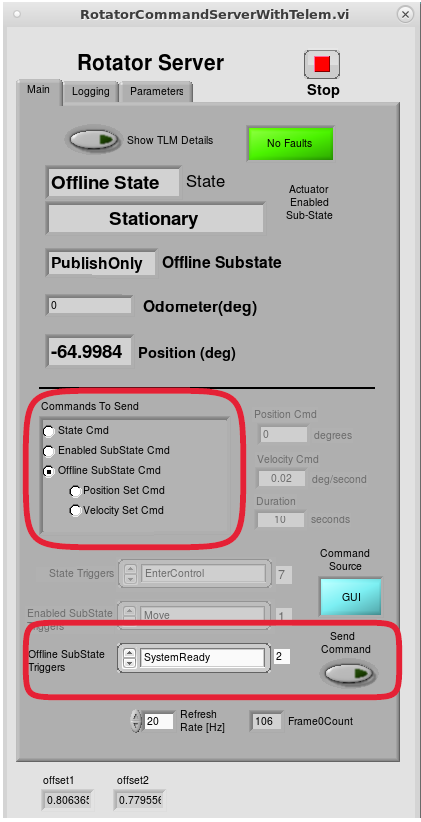
\includegraphics[width=1.79167in]{jira_imgs/1005.png}

\medskip }
\end{minipage}
\\ \cdashline{2-2}


 & Expected Result \\
 & \begin{minipage}[t]{15cm}{\footnotesize
\smallskip
The system transitions from the OfflineState/PublishOnly substate to the
OfflineState/AvailableState
substate.\\[2\baselineskip]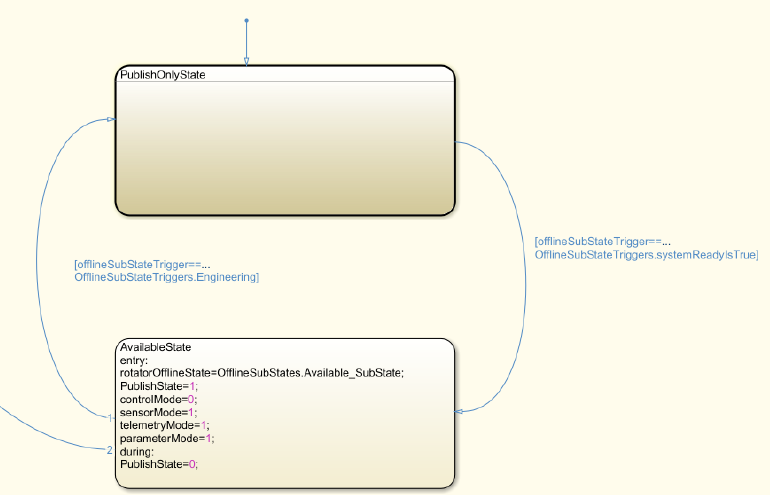
\includegraphics[width=1.79167in]{jira_imgs/1007.png}

\medskip }
\end{minipage} \\ \cdashline{2-2}

 & Actual Result \\
 & \begin{minipage}[t]{15cm}{\footnotesize
\smallskip

\medskip }
\end{minipage} \\ \cdashline{2-2}

 & Status: \textbf{ Pass } \\ \hline

4 & Description \\
 & \begin{minipage}[t]{15cm}
{\footnotesize
\smallskip
\textbf{SWITCHING TO DDS MODE}\\
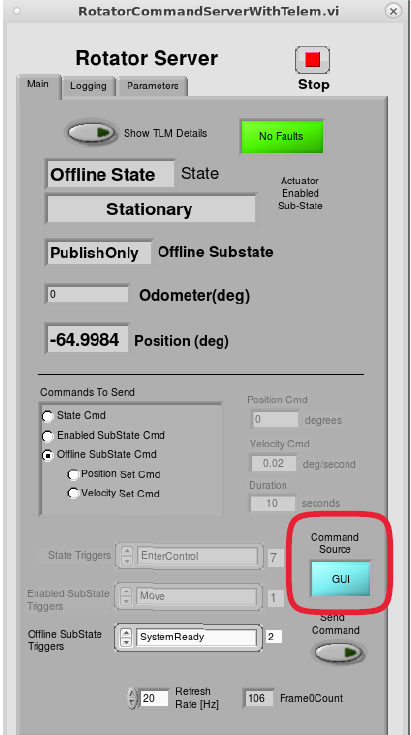
\includegraphics[width=1.79167in]{jira_imgs/1014.png}\\
If the Command Source does not show DDS, go to the Parameters tab,
select DDS under the Command Source and click the Set Command Source
button.\\
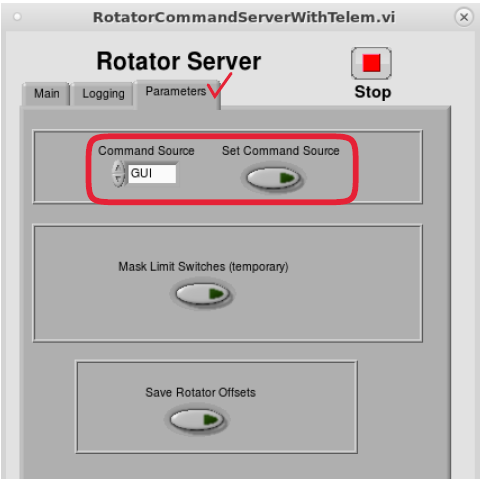
\includegraphics[width=1.79167in]{jira_imgs/1013.png}\textbf{Note:~If
the GUI is used after being set to DDS mode, the system will switch back
the Command Source to GUI and ignore any DDS commands. The Command
Source must show DDS in order to receive DDS commands.}

\medskip }
\end{minipage}
\\ \cdashline{2-2}


 & Expected Result \\
 & \begin{minipage}[t]{15cm}{\footnotesize
\smallskip
The system is capable of receiving/responding to DDS commands.

\medskip }
\end{minipage} \\ \cdashline{2-2}

 & Actual Result \\
 & \begin{minipage}[t]{15cm}{\footnotesize
\smallskip

\medskip }
\end{minipage} \\ \cdashline{2-2}

 & Status: \textbf{ Pass } \\ \hline

5 & Description \\
 & \begin{minipage}[t]{15cm}
{\footnotesize
\smallskip
\textbf{OFFLINESTATE -\textgreater{} STANDBYSTATE}\\
The system receives an enterControl State Transition command through
DDS.

\medskip }
\end{minipage}
\\ \cdashline{2-2}


 & Expected Result \\
 & \begin{minipage}[t]{15cm}{\footnotesize
\smallskip
The system transitions into the StandbyState and is capable of
receiving/responding to DDS commands.\\
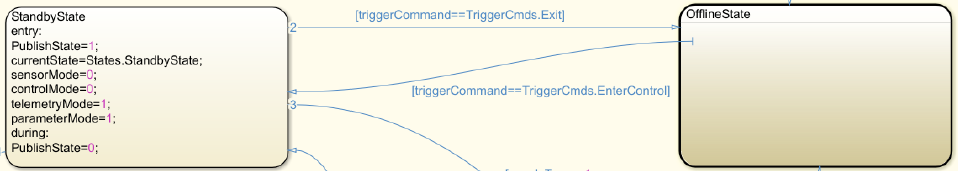
\includegraphics[width=4.68750in]{jira_imgs/1018.png}

\medskip }
\end{minipage} \\ \cdashline{2-2}

 & Actual Result \\
 & \begin{minipage}[t]{15cm}{\footnotesize
\smallskip

\medskip }
\end{minipage} \\ \cdashline{2-2}

 & Status: \textbf{ Not Executed } \\ \hline

6 & Description \\
 & \begin{minipage}[t]{15cm}
{\footnotesize
\smallskip
\textbf{STANDBYSTATE -\textgreater{} DISABLEDSTATE}\\
From the StandbyState, send a start command through the DDS.

\medskip }
\end{minipage}
\\ \cdashline{2-2}


 & Expected Result \\
 & \begin{minipage}[t]{15cm}{\footnotesize
\smallskip
The system transitions into DisabledState after receiving/responding to
DDS command and the wrapper in the PXI real time controller looks for
the configuration file.\\
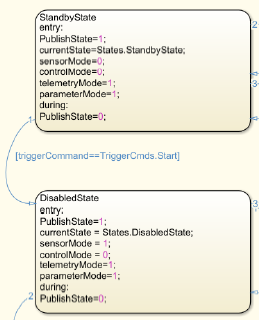
\includegraphics[width=1.79167in]{jira_imgs/1019.png}\\
If the configuration file is invalid or out of range, the system will
transition into a Fault State

\medskip }
\end{minipage} \\ \cdashline{2-2}

 & Actual Result \\
 & \begin{minipage}[t]{15cm}{\footnotesize
\smallskip

\medskip }
\end{minipage} \\ \cdashline{2-2}

 & Status: \textbf{ Not Executed } \\ \hline

7 & Description \\
 & \begin{minipage}[t]{15cm}
{\footnotesize
\smallskip
\textbf{DISABLEDSTATE -\textgreater{} ENABLEDSTATE}\\
From the DisabledState, send an enable state command through the DDS.\\
\textbf{}

\medskip }
\end{minipage}
\\ \cdashline{2-2}


 & Expected Result \\
 & \begin{minipage}[t]{15cm}{\footnotesize
\smallskip
The system transitions into the EnabledState/Stationary substate, the
motor drives are enabled, motor brakes are released and the system is
capable of receiving/responding to DDS commands.\\
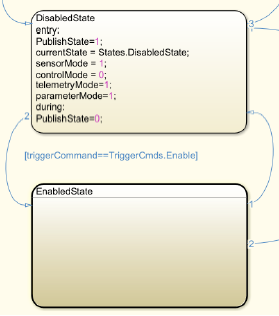
\includegraphics[width=1.79167in]{jira_imgs/1020.png}\\

\medskip }
\end{minipage} \\ \cdashline{2-2}

 & Actual Result \\
 & \begin{minipage}[t]{15cm}{\footnotesize
\smallskip

\medskip }
\end{minipage} \\ \cdashline{2-2}

 & Status: \textbf{ Not Executed } \\ \hline

8 & Description \\
 & \begin{minipage}[t]{15cm}
{\footnotesize
\smallskip
\textbf{FAULTSTATE}\\
If a Fault occurs in any of the other states, the system will
automatically transition to the Fault State. While in the Fault state,
send a clearError command through the DDS.\\
Note: If the fault that occurs goes through the interlock system, reset
the safety relay switch and send a clearError command.

\medskip }
\end{minipage}
\\ \cdashline{2-2}


 & Expected Result \\
 & \begin{minipage}[t]{15cm}{\footnotesize
\smallskip
The system transitions back to the OfflineState/PublishOnly substate and
is not capable of receiving/responding to DDS commands. (Go back to Step
3)\\
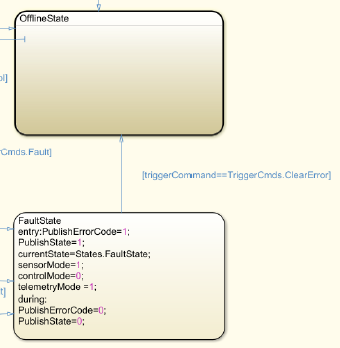
\includegraphics[width=1.79167in]{jira_imgs/1021.png}

\medskip }
\end{minipage} \\ \cdashline{2-2}

 & Actual Result \\
 & \begin{minipage}[t]{15cm}{\footnotesize
\smallskip

\medskip }
\end{minipage} \\ \cdashline{2-2}

 & Status: \textbf{ Not Executed } \\ \hline

9 & Description \\
 & \begin{minipage}[t]{15cm}
{\footnotesize
\smallskip
\textbf{GUI vs DDS Control}\\[2\baselineskip]While in DDS mode, send a
command from the EUI to test if an EUI user may take over control of the
camera rotator.

\medskip }
\end{minipage}
\\ \cdashline{2-2}


 & Expected Result \\
 & \begin{minipage}[t]{15cm}{\footnotesize
\smallskip
The system switches from DDS mode to GUI mode. The user must switch back
to the DDS Command Source through the GUI for the system to be
controlled through the CSC again.

\medskip }
\end{minipage} \\ \cdashline{2-2}

 & Actual Result \\
 & \begin{minipage}[t]{15cm}{\footnotesize
\smallskip

\medskip }
\end{minipage} \\ \cdashline{2-2}

 & Status: \textbf{ Not Executed } \\ \hline

10 & Description \\
 & \begin{minipage}[t]{15cm}
{\footnotesize
\smallskip
\textbf{Back To DDS Mode}\\
While the system is in GUI mode, go to the Parameters tab, select DDS
under the Command Source and click the Set Command Source
button\textbf{.~}

\medskip }
\end{minipage}
\\ \cdashline{2-2}


 & Expected Result \\
 & \begin{minipage}[t]{15cm}{\footnotesize
\smallskip
The system is capable of receiving/responding to DDS commands.

\medskip }
\end{minipage} \\ \cdashline{2-2}

 & Actual Result \\
 & \begin{minipage}[t]{15cm}{\footnotesize
\smallskip

\medskip }
\end{minipage} \\ \cdashline{2-2}

 & Status: \textbf{ Not Executed } \\ \hline

11 & Description \\
 & \begin{minipage}[t]{15cm}
{\footnotesize
\smallskip
\textbf{Section 3.2.2 of the attached Software Acceptance Test
Procedure\\
Test Sequence \#1 -- PositionSet and Move Commands}\\[2\baselineskip]In
the Enabled/Stationary state, send a positionSet command of 12 deg.

\medskip }
\end{minipage}
\\ \cdashline{2-2}


 & Expected Result \\
 & \begin{minipage}[t]{15cm}{\footnotesize
\smallskip
Confirm that the rotator does not move.

\medskip }
\end{minipage} \\ \cdashline{2-2}

 & Actual Result \\
 & \begin{minipage}[t]{15cm}{\footnotesize
\smallskip

\medskip }
\end{minipage} \\ \cdashline{2-2}

 & Status: \textbf{ Not Executed } \\ \hline

12 & Description \\
 & \begin{minipage}[t]{15cm}
{\footnotesize
\smallskip
Send a positionSet command of 15deg.

\medskip }
\end{minipage}
\\ \cdashline{2-2}


 & Expected Result \\
 & \begin{minipage}[t]{15cm}{\footnotesize
\smallskip
Confirm that the rotator does not move.

\medskip }
\end{minipage} \\ \cdashline{2-2}

 & Actual Result \\
 & \begin{minipage}[t]{15cm}{\footnotesize
\smallskip

\medskip }
\end{minipage} \\ \cdashline{2-2}

 & Status: \textbf{ Not Executed } \\ \hline

13 & Description \\
 & \begin{minipage}[t]{15cm}
{\footnotesize
\smallskip
Send a move command.\\[2\baselineskip]

\medskip }
\end{minipage}
\\ \cdashline{2-2}


 & Expected Result \\
 & \begin{minipage}[t]{15cm}{\footnotesize
\smallskip
Confirm that the rotator moves to 15deg and an inPosition event is
generated when the move is complete.

\medskip }
\end{minipage} \\ \cdashline{2-2}

 & Actual Result \\
 & \begin{minipage}[t]{15cm}{\footnotesize
\smallskip

\medskip }
\end{minipage} \\ \cdashline{2-2}

 & Status: \textbf{ Not Executed } \\ \hline

14 & Description \\
 & \begin{minipage}[t]{15cm}
{\footnotesize
\smallskip
Record the corresponding DDS events that were generated.

\medskip }
\end{minipage}
\\ \cdashline{2-2}


 & Expected Result \\
 & \begin{minipage}[t]{15cm}{\footnotesize
\smallskip
\begin{itemize}
\tightlist
\item
  The Application event outputs reasonable values
\item
  The controllerState.enabledSubstate goes to MOVING\_POINT\_TO\_POINT
  when the move begins and STATIONARY when the move ends
\end{itemize}

\medskip }
\end{minipage} \\ \cdashline{2-2}

 & Actual Result \\
 & \begin{minipage}[t]{15cm}{\footnotesize
\smallskip

\medskip }
\end{minipage} \\ \cdashline{2-2}

 & Status: \textbf{ Not Executed } \\ \hline

15 & Description \\
 & \begin{minipage}[t]{15cm}
{\footnotesize
\smallskip
\textbf{Section 3.2.2 of the attached Software Acceptance Test
Procedure\\
Test Sequence \#2 - Stop Command}\\[2\baselineskip]In the
Enabled/Stationary state, send a positionSet command of 50 deg.

\medskip }
\end{minipage}
\\ \cdashline{2-2}


 & Expected Result \\
 & \begin{minipage}[t]{15cm}{\footnotesize
\smallskip
Confirm that the rotator does not move.

\medskip }
\end{minipage} \\ \cdashline{2-2}

 & Actual Result \\
 & \begin{minipage}[t]{15cm}{\footnotesize
\smallskip

\medskip }
\end{minipage} \\ \cdashline{2-2}

 & Status: \textbf{ Not Executed } \\ \hline

16 & Description \\
 & \begin{minipage}[t]{15cm}
{\footnotesize
\smallskip
Send a move command.

\medskip }
\end{minipage}
\\ \cdashline{2-2}


 & Expected Result \\
 & \begin{minipage}[t]{15cm}{\footnotesize
\smallskip
The rotator starts its rotation.

\medskip }
\end{minipage} \\ \cdashline{2-2}

 & Actual Result \\
 & \begin{minipage}[t]{15cm}{\footnotesize
\smallskip

\medskip }
\end{minipage} \\ \cdashline{2-2}

 & Status: \textbf{ Not Executed } \\ \hline

17 & Description \\
 & \begin{minipage}[t]{15cm}
{\footnotesize
\smallskip
While the rotator is still moving, send a Stop command.

\medskip }
\end{minipage}
\\ \cdashline{2-2}


 & Expected Result \\
 & \begin{minipage}[t]{15cm}{\footnotesize
\smallskip
Confirm that the system quickly comes to a stop before reaching the 50
deg position.

\medskip }
\end{minipage} \\ \cdashline{2-2}

 & Actual Result \\
 & \begin{minipage}[t]{15cm}{\footnotesize
\smallskip

\medskip }
\end{minipage} \\ \cdashline{2-2}

 & Status: \textbf{ Not Executed } \\ \hline

18 & Description \\
 & \begin{minipage}[t]{15cm}
{\footnotesize
\smallskip
Send a positionSet command of 60 deg followed by a move command.

\medskip }
\end{minipage}
\\ \cdashline{2-2}


 & Expected Result \\
 & \begin{minipage}[t]{15cm}{\footnotesize
\smallskip
Confirm the rotator moves to the commanded position following the
previous stop command.

\medskip }
\end{minipage} \\ \cdashline{2-2}

 & Actual Result \\
 & \begin{minipage}[t]{15cm}{\footnotesize
\smallskip

\medskip }
\end{minipage} \\ \cdashline{2-2}

 & Status: \textbf{ Not Executed } \\ \hline

19 & Description \\
 & \begin{minipage}[t]{15cm}
{\footnotesize
\smallskip
Record the corresponding DDS events that were generated.

\medskip }
\end{minipage}
\\ \cdashline{2-2}


 & Expected Result \\
 & \begin{minipage}[t]{15cm}{\footnotesize
\smallskip
\begin{itemize}
\tightlist
\item
  The controllerState.enabledSubstate goes to CONTROLLED\_STOPPING when
  the stop is requested, then STATIONARY when the rotator has halted
\item
  The inPosition event is not reported as True.
\end{itemize}

\medskip }
\end{minipage} \\ \cdashline{2-2}

 & Actual Result \\
 & \begin{minipage}[t]{15cm}{\footnotesize
\smallskip

\medskip }
\end{minipage} \\ \cdashline{2-2}

 & Status: \textbf{ Not Executed } \\ \hline

20 & Description \\
 & \begin{minipage}[t]{15cm}
{\footnotesize
\smallskip
\textbf{Test of startTrack and track command}\\[2\baselineskip]In the
Enabled state, send a trackStart command. Do not send a Track command.

\medskip }
\end{minipage}
\\ \cdashline{2-2}


 & Expected Result \\
 & \begin{minipage}[t]{15cm}{\footnotesize
\smallskip
The cRIO goes into FAULT state without moving at all.

\medskip }
\end{minipage} \\ \cdashline{2-2}

 & Actual Result \\
 & \begin{minipage}[t]{15cm}{\footnotesize
\smallskip

\medskip }
\end{minipage} \\ \cdashline{2-2}

 & Status: \textbf{ Not Executed } \\ \hline

21 & Description \\
 & \begin{minipage}[t]{15cm}
{\footnotesize
\smallskip
\textbf{Section 3.2.2 of the attached Software Acceptance Test
Procedure\\
Test Sequence \#4 - Track and TrackStart Commands}\\[2\baselineskip]In
the Enabled/Stationary state, send a trackStart command.

\medskip }
\end{minipage}
\\ \cdashline{2-2}


 & Expected Result \\
 & \begin{minipage}[t]{15cm}{\footnotesize
\smallskip
Confirm that the system transitions into Enabled/Slewing and Tracking
state.

\medskip }
\end{minipage} \\ \cdashline{2-2}

 & Actual Result \\
 & \begin{minipage}[t]{15cm}{\footnotesize
\smallskip

\medskip }
\end{minipage} \\ \cdashline{2-2}

 & Status: \textbf{ Not Executed } \\ \hline

22 & Description \\
 & \begin{minipage}[t]{15cm}
{\footnotesize
\smallskip
Send a series of track commands at 20 Hz from
command\_vector\_set\_A.mat and ensure the system follows the commands
and sends appropriate tracking and trackLost events.

\medskip }
\end{minipage}
\\ \cdashline{2-2}

 & Test Data \\
 & \begin{minipage}[t]{15cm}{\footnotesize
\smallskip
\textbf{Deviation:} When the trackStart command is run, a track command
must be issued at 10-20Hz until tracking is done. The vendor's code
reads in a CSV file with tracking conditions when using the trackStart
command in order to circumvent a FAULT state due to lack of position,
velocity and time updates. Instead, use Russell's code which utilizes
the functions \emph{ramp~}and\emph{~sine~}to track from a start position
to an end position at a specified velocity and track along a sine wave,
respectively.

\medskip }
\end{minipage} \\ \cdashline{2-2}

 & Expected Result \\
 & \begin{minipage}[t]{15cm}{\footnotesize
\smallskip
The rotator first slews to meet the commanded path and then tracks that
path

\medskip }
\end{minipage} \\ \cdashline{2-2}

 & Actual Result \\
 & \begin{minipage}[t]{15cm}{\footnotesize
\smallskip

\medskip }
\end{minipage} \\ \cdashline{2-2}

 & Status: \textbf{ Not Executed } \\ \hline

23 & Description \\
 & \begin{minipage}[t]{15cm}
{\footnotesize
\smallskip
Record the corresponding DDS events that were generated.

\medskip }
\end{minipage}
\\ \cdashline{2-2}


 & Expected Result \\
 & \begin{minipage}[t]{15cm}{\footnotesize
\smallskip
\begin{itemize}
\tightlist
\item
  The Application event outputs reasonable values
\item
  The controllerState.enabledSubstate goes to SLEWING\_OR\_TRACKING when
  the move begins, CONTROLLED\_STOPPING when the movement sequence ends,
  and STATIONARY when the rotator has stopped
\item
  The inPosition event is True once slewing has finished and tracking
  begins
\end{itemize}

\medskip }
\end{minipage} \\ \cdashline{2-2}

 & Actual Result \\
 & \begin{minipage}[t]{15cm}{\footnotesize
\smallskip

\medskip }
\end{minipage} \\ \cdashline{2-2}

 & Status: \textbf{ Not Executed } \\ \hline

24 & Description \\
 & \begin{minipage}[t]{15cm}
{\footnotesize
\smallskip
\textbf{Section 3.2.2 of the attached Software Acceptance Test
Procedure\\
Test Sequence \#5 - Track and TrackStart Commands}\\[2\baselineskip]In
the Enabled/Stationary state, send a trackStart command.

\medskip }
\end{minipage}
\\ \cdashline{2-2}


 & Expected Result \\
 & \begin{minipage}[t]{15cm}{\footnotesize
\smallskip
Confirm that the system transitions into Enabled/Slewing and Tracking
state.

\medskip }
\end{minipage} \\ \cdashline{2-2}

 & Actual Result \\
 & \begin{minipage}[t]{15cm}{\footnotesize
\smallskip

\medskip }
\end{minipage} \\ \cdashline{2-2}

 & Status: \textbf{ Not Executed } \\ \hline

25 & Description \\
 & \begin{minipage}[t]{15cm}
{\footnotesize
\smallskip
Send a series of track commands at 20 Hz from
command\_vector\_set\_B.mat and ensure the system follows the commands
and sends appropriate tracking and trackLost events.

\medskip }
\end{minipage}
\\ \cdashline{2-2}

 & Test Data \\
 & \begin{minipage}[t]{15cm}{\footnotesize
\smallskip
\textbf{Deviation:} When the trackStart command is run, a track command
must be issued at 10-20Hz until tracking is done. The vendor's code
reads in a CSV file with tracking conditions when using the trackStart
command in order to circumvent a FAULT state due to lack of position,
velocity and time updates. Instead, use Russell's code which utilizes
the functions \emph{ramp~}and\emph{~sine~}to track from a start position
to an end position at a specified velocity and track along a sine wave,
respectively.

\medskip }
\end{minipage} \\ \cdashline{2-2}

 & Expected Result \\
 & \begin{minipage}[t]{15cm}{\footnotesize
\smallskip
The rotator first slews to meet the commanded path and then tracks that
path

\medskip }
\end{minipage} \\ \cdashline{2-2}

 & Actual Result \\
 & \begin{minipage}[t]{15cm}{\footnotesize
\smallskip

\medskip }
\end{minipage} \\ \cdashline{2-2}

 & Status: \textbf{ Not Executed } \\ \hline

26 & Description \\
 & \begin{minipage}[t]{15cm}
{\footnotesize
\smallskip
Record the corresponding DDS events that were generated.

\medskip }
\end{minipage}
\\ \cdashline{2-2}


 & Expected Result \\
 & \begin{minipage}[t]{15cm}{\footnotesize
\smallskip
\begin{itemize}
\tightlist
\item
  The Application event outputs reasonable values
\item
  The controllerState.enabledSubstate goes to SLEWING\_OR\_TRACKING when
  the move begins, CONTROLLED\_STOPPING when the movement sequence ends,
  and STATIONARY when the rotator has stopped
\item
  The inPosition event is True once slewing has finished and tracking
  begins
\end{itemize}

\medskip }
\end{minipage} \\ \cdashline{2-2}

 & Actual Result \\
 & \begin{minipage}[t]{15cm}{\footnotesize
\smallskip

\medskip }
\end{minipage} \\ \cdashline{2-2}

 & Status: \textbf{ Not Executed } \\ \hline

27 & Description \\
 & \begin{minipage}[t]{15cm}
{\footnotesize
\smallskip
\textbf{Section 3.2.2 of the attached Software Acceptance Test
Procedure\\
Test Sequence \#6 - configureVelocity Command}\\[2\baselineskip]In the
Enabled/Stationary state, send a configureVelocity command of 4 deg/s.

\medskip }
\end{minipage}
\\ \cdashline{2-2}


 & Expected Result \\
 & \begin{minipage}[t]{15cm}{\footnotesize
\smallskip
Confirm that the command is rejected for being out of acceptable range.

\medskip }
\end{minipage} \\ \cdashline{2-2}

 & Actual Result \\
 & \begin{minipage}[t]{15cm}{\footnotesize
\smallskip

\medskip }
\end{minipage} \\ \cdashline{2-2}

 & Status: \textbf{ Not Executed } \\ \hline

28 & Description \\
 & \begin{minipage}[t]{15cm}
{\footnotesize
\smallskip
Send a configureVelocity command of 0.5 deg/s.

\medskip }
\end{minipage}
\\ \cdashline{2-2}


 & Expected Result \\
 & \begin{minipage}[t]{15cm}{\footnotesize
\smallskip
Confirm that this command is accepted.

\medskip }
\end{minipage} \\ \cdashline{2-2}

 & Actual Result \\
 & \begin{minipage}[t]{15cm}{\footnotesize
\smallskip

\medskip }
\end{minipage} \\ \cdashline{2-2}

 & Status: \textbf{ Not Executed } \\ \hline

29 & Description \\
 & \begin{minipage}[t]{15cm}
{\footnotesize
\smallskip
Send a positionSet command to a position 10 deg away from the current
position. Send a move command.

\medskip }
\end{minipage}
\\ \cdashline{2-2}


 & Expected Result \\
 & \begin{minipage}[t]{15cm}{\footnotesize
\smallskip
Confirm the that move in completed in approximately 20 seconds.

\medskip }
\end{minipage} \\ \cdashline{2-2}

 & Actual Result \\
 & \begin{minipage}[t]{15cm}{\footnotesize
\smallskip

\medskip }
\end{minipage} \\ \cdashline{2-2}

 & Status: \textbf{ Not Executed } \\ \hline

30 & Description \\
 & \begin{minipage}[t]{15cm}
{\footnotesize
\smallskip
Record the corresponding DDS events that were generated.

\medskip }
\end{minipage}
\\ \cdashline{2-2}


 & Expected Result \\
 & \begin{minipage}[t]{15cm}{\footnotesize
\smallskip
\begin{itemize}
\tightlist
\item
  The Application event outputs reasonable values
\item
  The controllerState.enabledSubstate goes to MOVING\_POINT\_TO\_POINT
  when the move begins and STATIONARY when the move ends
\item
  The inPosition event is True once move has finished
\end{itemize}

\medskip }
\end{minipage} \\ \cdashline{2-2}

 & Actual Result \\
 & \begin{minipage}[t]{15cm}{\footnotesize
\smallskip

\medskip }
\end{minipage} \\ \cdashline{2-2}

 & Status: \textbf{ Not Executed } \\ \hline

31 & Description \\
 & \begin{minipage}[t]{15cm}
{\footnotesize
\smallskip
\textbf{Section 3.2.2 of the attached Software Acceptance Test
Procedure\\
Test Sequence \#7 - configureAcceleration Command}\\[2\baselineskip]In
the Enabled/Stationary state with the configureVelocity command from the
previous test still in effect, send a configureAcceleration command of 2
deg/s\^{}2.

\medskip }
\end{minipage}
\\ \cdashline{2-2}


 & Expected Result \\
 & \begin{minipage}[t]{15cm}{\footnotesize
\smallskip
Confirm that the command is rejected for being out of acceptable range.

\medskip }
\end{minipage} \\ \cdashline{2-2}

 & Actual Result \\
 & \begin{minipage}[t]{15cm}{\footnotesize
\smallskip

\medskip }
\end{minipage} \\ \cdashline{2-2}

 & Status: \textbf{ Not Executed } \\ \hline

32 & Description \\
 & \begin{minipage}[t]{15cm}
{\footnotesize
\smallskip
Send a configureAcceleration command of 0.05 deg/s\^{}2.

\medskip }
\end{minipage}
\\ \cdashline{2-2}


 & Expected Result \\
 & \begin{minipage}[t]{15cm}{\footnotesize
\smallskip
Confirm that the command is accepted.

\medskip }
\end{minipage} \\ \cdashline{2-2}

 & Actual Result \\
 & \begin{minipage}[t]{15cm}{\footnotesize
\smallskip

\medskip }
\end{minipage} \\ \cdashline{2-2}

 & Status: \textbf{ Not Executed } \\ \hline

33 & Description \\
 & \begin{minipage}[t]{15cm}
{\footnotesize
\smallskip
Send a positionSet command to a position 10 deg away from the current
position. Send a move command.

\medskip }
\end{minipage}
\\ \cdashline{2-2}


 & Expected Result \\
 & \begin{minipage}[t]{15cm}{\footnotesize
\smallskip
Confirm the that move in completed in approximately 30 seconds.

\medskip }
\end{minipage} \\ \cdashline{2-2}

 & Actual Result \\
 & \begin{minipage}[t]{15cm}{\footnotesize
\smallskip

\medskip }
\end{minipage} \\ \cdashline{2-2}

 & Status: \textbf{ Not Executed } \\ \hline

34 & Description \\
 & \begin{minipage}[t]{15cm}
{\footnotesize
\smallskip
Record the corresponding DDS events that were generated.

\medskip }
\end{minipage}
\\ \cdashline{2-2}


 & Expected Result \\
 & \begin{minipage}[t]{15cm}{\footnotesize
\smallskip
\begin{itemize}
\tightlist
\item
  The Application event outputs reasonable values
\item
  The controllerState.enabledSubstate goes to MOVING\_POINT\_TO\_POINT
  when the move begins and STATIONARY when the move ends
\item
  The inPosition event is True once move has finished
\end{itemize}

\medskip }
\end{minipage} \\ \cdashline{2-2}

 & Actual Result \\
 & \begin{minipage}[t]{15cm}{\footnotesize
\smallskip

\medskip }
\end{minipage} \\ \cdashline{2-2}

 & Status: \textbf{ Not Executed } \\ \hline

35 & Description \\
 & \begin{minipage}[t]{15cm}
{\footnotesize
\smallskip
Shutdown the rotator.

\medskip }
\end{minipage}
\\ \cdashline{2-2}


 & Expected Result \\
 & \begin{minipage}[t]{15cm}{\footnotesize
\smallskip
Rotator is shutdown.

\medskip }
\end{minipage} \\ \cdashline{2-2}

 & Actual Result \\
 & \begin{minipage}[t]{15cm}{\footnotesize
\smallskip

\medskip }
\end{minipage} \\ \cdashline{2-2}

 & Status: \textbf{ Not Executed } \\ \hline

36 & Description \\
 & \begin{minipage}[t]{15cm}
{\footnotesize
\smallskip
\textbf{Section 3.3.2 of the attached Software Acceptance Test
Procedure}\\
\textbf{Rotator Action on State Commands\\
}\\
Start up the system.

\medskip }
\end{minipage}
\\ \cdashline{2-2}


 & Expected Result \\
 & \begin{minipage}[t]{15cm}{\footnotesize
\smallskip
\begin{itemize}
\tightlist
\item
  Confirm the system starts up in Offline/PublishOnly state.
\item
  When the middleware starts up, confirm that a SettingsVersions event
  is published with a list of all saved settings file names and a
  settingsApplied event is published with a list of all default
  configurable parameters.
\end{itemize}

\medskip }
\end{minipage} \\ \cdashline{2-2}

 & Actual Result \\
 & \begin{minipage}[t]{15cm}{\footnotesize
\smallskip

\medskip }
\end{minipage} \\ \cdashline{2-2}

 & Status: \textbf{ Not Executed } \\ \hline

37 & Description \\
 & \begin{minipage}[t]{15cm}
{\footnotesize
\smallskip
Send the enterControl command.

\medskip }
\end{minipage}
\\ \cdashline{2-2}


 & Expected Result \\
 & \begin{minipage}[t]{15cm}{\footnotesize
\smallskip
Confirm that the system does not respond to a EnterControl command over
DDS.

\medskip }
\end{minipage} \\ \cdashline{2-2}

 & Actual Result \\
 & \begin{minipage}[t]{15cm}{\footnotesize
\smallskip

\medskip }
\end{minipage} \\ \cdashline{2-2}

 & Status: \textbf{ Not Executed } \\ \hline

38 & Description \\
 & \begin{minipage}[t]{15cm}
{\footnotesize
\smallskip
From the EUI send an offline substate trigger of systemReady.

\medskip }
\end{minipage}
\\ \cdashline{2-2}


 & Expected Result \\
 & \begin{minipage}[t]{15cm}{\footnotesize
\smallskip
Confirm system goes into Offline/Available substate.

\medskip }
\end{minipage} \\ \cdashline{2-2}

 & Actual Result \\
 & \begin{minipage}[t]{15cm}{\footnotesize
\smallskip

\medskip }
\end{minipage} \\ \cdashline{2-2}

 & Status: \textbf{ Not Executed } \\ \hline

39 & Description \\
 & \begin{minipage}[t]{15cm}
{\footnotesize
\smallskip
From the EUI, select the DDS button to allow the system to receive
commands from DDS.

\medskip }
\end{minipage}
\\ \cdashline{2-2}


 & Expected Result \\
 & \begin{minipage}[t]{15cm}{\footnotesize
\smallskip
The EUI displays you are in DDS command mode.

\medskip }
\end{minipage} \\ \cdashline{2-2}

 & Actual Result \\
 & \begin{minipage}[t]{15cm}{\footnotesize
\smallskip

\medskip }
\end{minipage} \\ \cdashline{2-2}

 & Status: \textbf{ Not Executed } \\ \hline

40 & Description \\
 & \begin{minipage}[t]{15cm}
{\footnotesize
\smallskip
Send an EnterControl trigger. Record the corresponding DDS event(s) that
were generated.

\medskip }
\end{minipage}
\\ \cdashline{2-2}


 & Expected Result \\
 & \begin{minipage}[t]{15cm}{\footnotesize
\smallskip
Confirm the system transitions from Offline/Available to Standby state.

\medskip }
\end{minipage} \\ \cdashline{2-2}

 & Actual Result \\
 & \begin{minipage}[t]{15cm}{\footnotesize
\smallskip

\medskip }
\end{minipage} \\ \cdashline{2-2}

 & Status: \textbf{ Not Executed } \\ \hline

41 & Description \\
 & \begin{minipage}[t]{15cm}
{\footnotesize
\smallskip
Send a Start trigger with an invalid filename.

\medskip }
\end{minipage}
\\ \cdashline{2-2}


 & Expected Result \\
 & \begin{minipage}[t]{15cm}{\footnotesize
\smallskip
Verify that the command is rejected and the system does not transition
out of Standby state.

\medskip }
\end{minipage} \\ \cdashline{2-2}

 & Actual Result \\
 & \begin{minipage}[t]{15cm}{\footnotesize
\smallskip

\medskip }
\end{minipage} \\ \cdashline{2-2}

 & Status: \textbf{ Not Executed } \\ \hline

42 & Description \\
 & \begin{minipage}[t]{15cm}
{\footnotesize
\smallskip
Send a Start trigger with a valid filename. Record the corresponding DDS
event(s) that were generated.

\medskip }
\end{minipage}
\\ \cdashline{2-2}


 & Expected Result \\
 & \begin{minipage}[t]{15cm}{\footnotesize
\smallskip
Confirm the system transitions from Standby to Disabled state and a
settingApplied and AppliedSettingsMatchStart = True events are
generated.

\medskip }
\end{minipage} \\ \cdashline{2-2}

 & Actual Result \\
 & \begin{minipage}[t]{15cm}{\footnotesize
\smallskip

\medskip }
\end{minipage} \\ \cdashline{2-2}

 & Status: \textbf{ Not Executed } \\ \hline

43 & Description \\
 & \begin{minipage}[t]{15cm}
{\footnotesize
\smallskip
Send an Enable trigger. Record the corresponding DDS event(s) that were
generated.

\medskip }
\end{minipage}
\\ \cdashline{2-2}


 & Expected Result \\
 & \begin{minipage}[t]{15cm}{\footnotesize
\smallskip
Confirm the system transitions from Disabled to Enabled state.

\medskip }
\end{minipage} \\ \cdashline{2-2}

 & Actual Result \\
 & \begin{minipage}[t]{15cm}{\footnotesize
\smallskip

\medskip }
\end{minipage} \\ \cdashline{2-2}

 & Status: \textbf{ Not Executed } \\ \hline

44 & Description \\
 & \begin{minipage}[t]{15cm}
{\footnotesize
\smallskip
Send a Disable trigger. Record the corresponding DDS event(s) that were
generated.

\medskip }
\end{minipage}
\\ \cdashline{2-2}


 & Expected Result \\
 & \begin{minipage}[t]{15cm}{\footnotesize
\smallskip
Confirm the system transitions from Enabled to Disabled state.

\medskip }
\end{minipage} \\ \cdashline{2-2}

 & Actual Result \\
 & \begin{minipage}[t]{15cm}{\footnotesize
\smallskip

\medskip }
\end{minipage} \\ \cdashline{2-2}

 & Status: \textbf{ Not Executed } \\ \hline

45 & Description \\
 & \begin{minipage}[t]{15cm}
{\footnotesize
\smallskip
Send a Standby trigger. Record the corresponding DDS event(s) that were
generated.

\medskip }
\end{minipage}
\\ \cdashline{2-2}


 & Expected Result \\
 & \begin{minipage}[t]{15cm}{\footnotesize
\smallskip
Confirm the system transitions from Disabled state to Standby state.

\medskip }
\end{minipage} \\ \cdashline{2-2}

 & Actual Result \\
 & \begin{minipage}[t]{15cm}{\footnotesize
\smallskip

\medskip }
\end{minipage} \\ \cdashline{2-2}

 & Status: \textbf{ Not Executed } \\ \hline

46 & Description \\
 & \begin{minipage}[t]{15cm}
{\footnotesize
\smallskip
Send a exitControl trigger. Record the corresponding DDS event(s) that
were generated.

\medskip }
\end{minipage}
\\ \cdashline{2-2}


 & Expected Result \\
 & \begin{minipage}[t]{15cm}{\footnotesize
\smallskip
Confirm the system transitions from Standby state to Offline state.

\medskip }
\end{minipage} \\ \cdashline{2-2}

 & Actual Result \\
 & \begin{minipage}[t]{15cm}{\footnotesize
\smallskip

\medskip }
\end{minipage} \\ \cdashline{2-2}

 & Status: \textbf{ Not Executed } \\ \hline

47 & Description \\
 & \begin{minipage}[t]{15cm}
{\footnotesize
\smallskip
\textbf{Section 5.1 of the attached Software Acceptance Test
Procedure}\\
\textbf{Rotator Events\\
}\\
In the Enabled state, unplug an encoder cable for one of the rotator
motors.

\medskip }
\end{minipage}
\\ \cdashline{2-2}

 & Test Data \\
 & \begin{minipage}[t]{15cm}{\footnotesize
\smallskip
\textbf{NOTE:} After each step in this set of steps, we will need to
send the clearError command to the CSC. This will put the cRIO into
Offline/PublishOnly. Use the EUI to re-enable CSC control.

\medskip }
\end{minipage} \\ \cdashline{2-2}

 & Expected Result \\
 & \begin{minipage}[t]{15cm}{\footnotesize
\smallskip
Confirm that a Drive Fault event is created and the system transitions
to Fault state.

\medskip }
\end{minipage} \\ \cdashline{2-2}

 & Actual Result \\
 & \begin{minipage}[t]{15cm}{\footnotesize
\smallskip

\medskip }
\end{minipage} \\ \cdashline{2-2}

 & Status: \textbf{ Not Executed } \\ \hline

48 & Description \\
 & \begin{minipage}[t]{15cm}
{\footnotesize
\smallskip
In the Enabled state, unplug a linear encoder cable for the rotator.

\medskip }
\end{minipage}
\\ \cdashline{2-2}


 & Expected Result \\
 & \begin{minipage}[t]{15cm}{\footnotesize
\smallskip
Confirm that a Linear Encoder Error event is created and the system
transitions to Fault state.

\medskip }
\end{minipage} \\ \cdashline{2-2}

 & Actual Result \\
 & \begin{minipage}[t]{15cm}{\footnotesize
\smallskip

\medskip }
\end{minipage} \\ \cdashline{2-2}

 & Status: \textbf{ Not Executed } \\ \hline

49 & Description \\
 & \begin{minipage}[t]{15cm}
{\footnotesize
\smallskip
Set the Following Error Threshold parameter to a very small value
(0.0001 deg or smaller) and command a PositionSet/Move.

\medskip }
\end{minipage}
\\ \cdashline{2-2}


 & Expected Result \\
 & \begin{minipage}[t]{15cm}{\footnotesize
\smallskip
Confirm that a Following Error event is created and the system
transitions to Fault state.

\medskip }
\end{minipage} \\ \cdashline{2-2}

 & Actual Result \\
 & \begin{minipage}[t]{15cm}{\footnotesize
\smallskip

\medskip }
\end{minipage} \\ \cdashline{2-2}

 & Status: \textbf{ Not Executed } \\ \hline

50 & Description \\
 & \begin{minipage}[t]{15cm}
{\footnotesize
\smallskip
Activate the positive software limit using a special control program.

\medskip }
\end{minipage}
\\ \cdashline{2-2}


 & Expected Result \\
 & \begin{minipage}[t]{15cm}{\footnotesize
\smallskip
Confirm that a Positive Limit Switch error message is created and the
system transitions to Fault state.

\medskip }
\end{minipage} \\ \cdashline{2-2}

 & Actual Result \\
 & \begin{minipage}[t]{15cm}{\footnotesize
\smallskip

\medskip }
\end{minipage} \\ \cdashline{2-2}

 & Status: \textbf{ Not Executed } \\ \hline

51 & Description \\
 & \begin{minipage}[t]{15cm}
{\footnotesize
\smallskip
Activate the negative software limit using a special control program.

\medskip }
\end{minipage}
\\ \cdashline{2-2}


 & Expected Result \\
 & \begin{minipage}[t]{15cm}{\footnotesize
\smallskip
Confirm that a Negative Limit Switch error message is created and the
system transitions to Fault State.

\medskip }
\end{minipage} \\ \cdashline{2-2}

 & Actual Result \\
 & \begin{minipage}[t]{15cm}{\footnotesize
\smallskip

\medskip }
\end{minipage} \\ \cdashline{2-2}

 & Status: \textbf{ Not Executed } \\ \hline

52 & Description \\
 & \begin{minipage}[t]{15cm}
{\footnotesize
\smallskip
Unplug the Ethercat cable between the control PC and the Copley XE2
drive.

\medskip }
\end{minipage}
\\ \cdashline{2-2}


 & Expected Result \\
 & \begin{minipage}[t]{15cm}{\footnotesize
\smallskip
Confirm that an Ethercat Problem event is created and the system
transitions to Fault state.

\medskip }
\end{minipage} \\ \cdashline{2-2}

 & Actual Result \\
 & \begin{minipage}[t]{15cm}{\footnotesize
\smallskip

\medskip }
\end{minipage} \\ \cdashline{2-2}

 & Status: \textbf{ Not Executed } \\ \hline

53 & Description \\
 & \begin{minipage}[t]{15cm}
{\footnotesize
\smallskip
Shutdown the rotator.

\medskip }
\end{minipage}
\\ \cdashline{2-2}


 & Expected Result \\
 & \begin{minipage}[t]{15cm}{\footnotesize
\smallskip
Rotator is shutdown.

\medskip }
\end{minipage} \\ \cdashline{2-2}

 & Actual Result \\
 & \begin{minipage}[t]{15cm}{\footnotesize
\smallskip

\medskip }
\end{minipage} \\ \cdashline{2-2}

 & Status: \textbf{ Not Executed } \\ \hline

\end{longtable}

\paragraph{Test Case LVV-T1569 - Integrated CCW + HR Interlock Test
 }\mbox{}\\

Open  \href{https://jira.lsstcorp.org/secure/Tests.jspa#/testCase/LVV-T1569}{\textit{ LVV-T1569 } }
test case in Jira.

The objective of this test case is to verify the interlocks of the
integrated CCW and Camera Rotator. This test case will exercise the
functionality of the combined interlock system between the CCW and the
Camera Rotator and meets the following criteria:

\begin{itemize}
\tightlist
\item
  Requires CCW AUX IS to be connected to the Camera Rotator IS
\item
  Requires WOBBLE assembly to be electrically and mechanically connected
\item
  Does \textbf{NOT} require the camera rotator to be loaded with the
  camera simulated mass or actual camera hardware
\item
  Does \textbf{NOT~}require CCW and Camera Rotator to be under combined
  control
\end{itemize}

The interlock system requirements for the Camera Rotator were previously
verified during the software functional re-verification test at the
summit facility. The test procedure used during the re-verification
testing is the \emph{LSST Hexapods-Rotator Software Acceptance Test
Procedure} which is attached to this test case. This includes the
procedure that covered how the interlocks were triggered for the Camera
Rotator, however it is a different configuration with the CCW
integrated.


\textbf{ Preconditions}:\\
Prior to the execution of this test case to verify the interlocks of the
CCW + HR, the following Summit tasks must be completed:\\

\begin{itemize}
\tightlist
\item
  The CCW has been installed on the Camera Cart

  \begin{itemize}
  \tightlist
  \item
    \url{https://jira.lsstcorp.org/browse/SUMMIT-2156}
  \end{itemize}
\item
  The functional testing of the Camera Rotator Hardware~

  \begin{itemize}
  \tightlist
  \item
    h\href{https://jira.lsstcorp.org/browse/SUMMIT-3370}{ttps://jira.lsstcorp.org/browse/SUMMIT-3370}
  \end{itemize}
\item
  The functional testing of the Camera Rotator Software without SAL

  \begin{itemize}
  \tightlist
  \item
    \url{https://jira.lsstcorp.org/browse/SUMMIT-3371}
  \end{itemize}
\item
  The Camera rotator has been connected to the electronics cabinets and
  the connections have been tested

  \begin{itemize}
  \tightlist
  \item
    \url{https://jira.lsstcorp.org/browse/SUMMIT-3294}
  \end{itemize}
\item
  The Hexapod and Rotator have been installed on camera cart

  \begin{itemize}
  \tightlist
  \item
    \url{https://jira.lsstcorp.org/browse/SUMMIT-3224}
  \end{itemize}
\item
  The cables and cabinets have been checked

  \begin{itemize}
  \tightlist
  \item
    \url{https://jira.lsstcorp.org/browse/SUMMIT-3231}
  \end{itemize}
\end{itemize}


Execution status: {\bf Not Executed }

Final comment:\\


Detailed steps results:

\begin{longtable}{p{1cm}p{15cm}}
\hline
{Step} & Step Details\\ \hline
1 & Description \\
 & \begin{minipage}[t]{15cm}
{\footnotesize
\smallskip
\textbf{STARTING THE EUI}\\[2\baselineskip]Double click the Hexapod GUI
Viewer desktop icon on the computer.

\begin{itemize}
\tightlist
\item
  This can be done on the Dell Management PC or another computer on the
  same network
\end{itemize}

\medskip }
\end{minipage}
\\ \cdashline{2-2}


 & Expected Result \\
 & \begin{minipage}[t]{15cm}{\footnotesize
\smallskip
A prompt to enter a password is shown.~

\medskip }
\end{minipage} \\ \cdashline{2-2}

 & Actual Result \\
 & \begin{minipage}[t]{15cm}{\footnotesize
\smallskip

\medskip }
\end{minipage} \\ \cdashline{2-2}

 & Status: \textbf{ Not Executed } \\ \hline

2 & Description \\
 & \begin{minipage}[t]{15cm}
{\footnotesize
\smallskip
Enter the password ``lsst-vnc''

\begin{itemize}
\tightlist
\item
  If the EUI isn't automatically up and running when the VNC opens,
  double click on the CAM\_Hex\_eGUI or M2\_Hex\_eGUI icon on the VNC
  viewer
\end{itemize}

\medskip }
\end{minipage}
\\ \cdashline{2-2}


 & Expected Result \\
 & \begin{minipage}[t]{15cm}{\footnotesize
\smallskip
The EUI is in the Offline State/PublishOnly substate and is able to
publish through SAL but cannot receive commands.

\medskip }
\end{minipage} \\ \cdashline{2-2}

 & Actual Result \\
 & \begin{minipage}[t]{15cm}{\footnotesize
\smallskip

\medskip }
\end{minipage} \\ \cdashline{2-2}

 & Status: \textbf{ Not Executed } \\ \hline

3 & Description \\
 & \begin{minipage}[t]{15cm}
{\footnotesize
\smallskip
\textbf{OFFLINESTATE/AVAILABLESTATE}\\
On the Main tab, select the ``Offline SubState Cmd'' field in the
Commands to Send section, set the Offline SubState Triggers to ``System
Ready'' and click on the Send Command button.\\
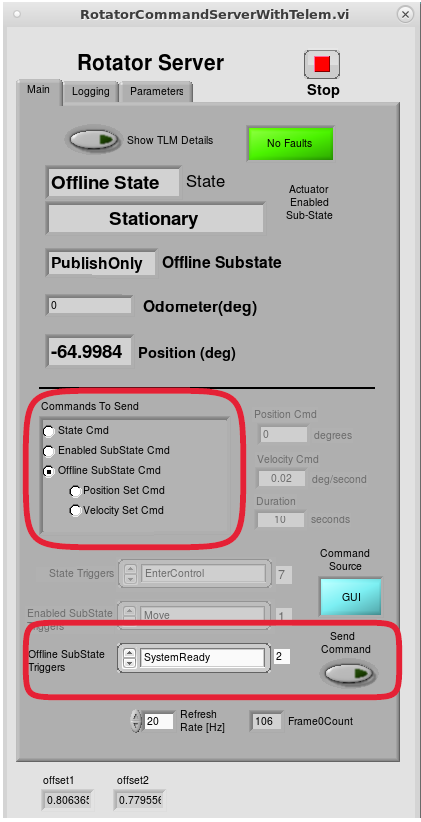
\includegraphics[width=1.79167in]{jira_imgs/1005.png}

\medskip }
\end{minipage}
\\ \cdashline{2-2}


 & Expected Result \\
 & \begin{minipage}[t]{15cm}{\footnotesize
\smallskip
The system transitions from the OfflineState/PublishOnly substate to the
OfflineState/AvailableState
substate.\\[2\baselineskip]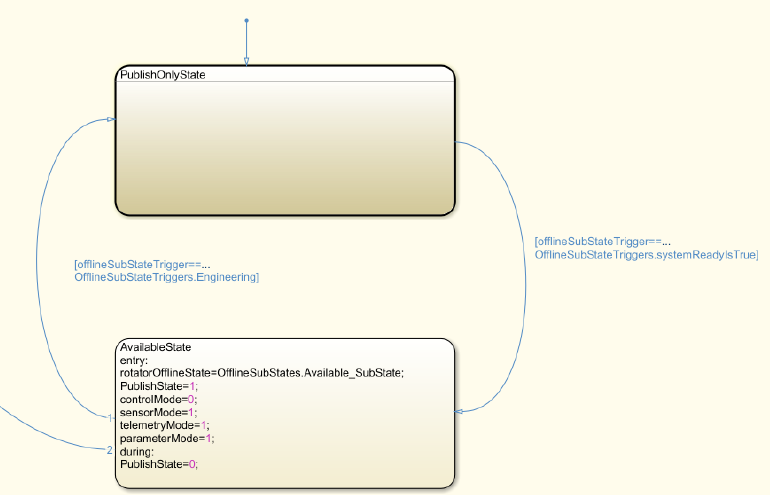
\includegraphics[width=1.79167in]{jira_imgs/1007.png}

\medskip }
\end{minipage} \\ \cdashline{2-2}

 & Actual Result \\
 & \begin{minipage}[t]{15cm}{\footnotesize
\smallskip

\medskip }
\end{minipage} \\ \cdashline{2-2}

 & Status: \textbf{ Not Executed } \\ \hline

4 & Description \\
 & \begin{minipage}[t]{15cm}
{\footnotesize
\smallskip
\textbf{SWITCHING TO DDS MODE}\\
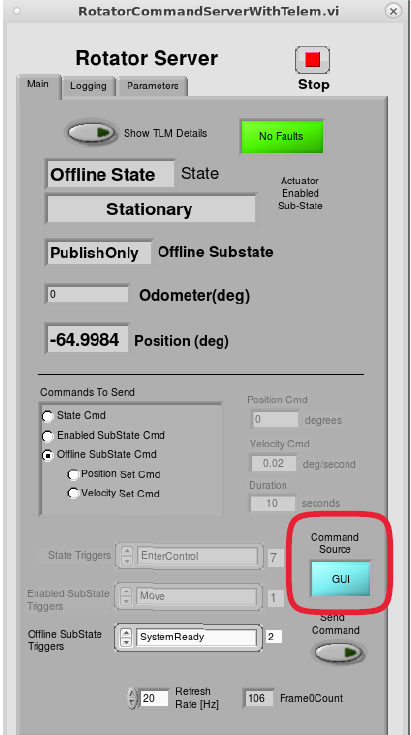
\includegraphics[width=1.79167in]{jira_imgs/1014.png}\\
If the Command Source does not show DDS, go to the Parameters tab,
select DDS under the Command Source and click the Set Command Source
button.\\
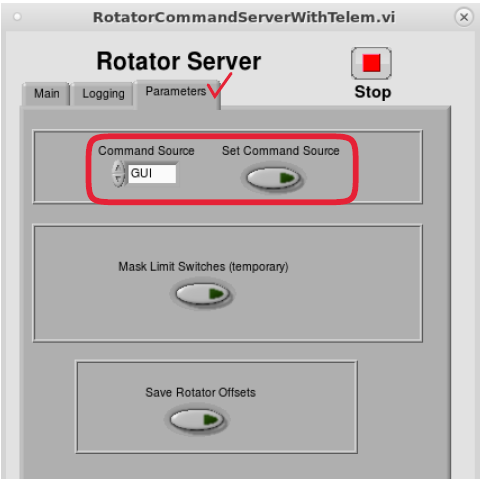
\includegraphics[width=1.79167in]{jira_imgs/1013.png}\textbf{Note:~If
the GUI is used after being set to DDS mode, the system will switch back
the Command Source to GUI and ignore any DDS commands. The Command
Source must show DDS in order to receive DDS commands.}

\medskip }
\end{minipage}
\\ \cdashline{2-2}


 & Expected Result \\
 & \begin{minipage}[t]{15cm}{\footnotesize
\smallskip
The system is capable of receiving/responding to DDS commands.

\medskip }
\end{minipage} \\ \cdashline{2-2}

 & Actual Result \\
 & \begin{minipage}[t]{15cm}{\footnotesize
\smallskip

\medskip }
\end{minipage} \\ \cdashline{2-2}

 & Status: \textbf{ Not Executed } \\ \hline

5 & Description \\
 & \begin{minipage}[t]{15cm}
{\footnotesize
\smallskip
\textbf{OFFLINESTATE -\textgreater{} STANDBYSTATE}\\
The system receives an enterControl State Transition command through
DDS.

\medskip }
\end{minipage}
\\ \cdashline{2-2}


 & Expected Result \\
 & \begin{minipage}[t]{15cm}{\footnotesize
\smallskip
The system transitions into the StandbyState and is capable of
receiving/responding to DDS commands.\\
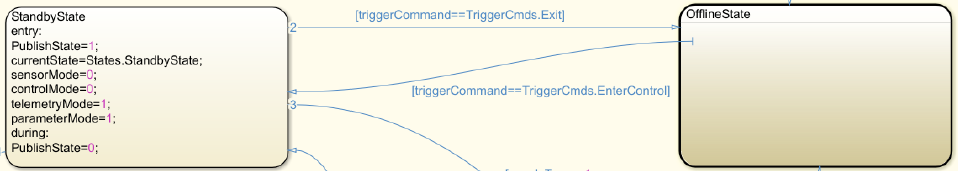
\includegraphics[width=4.68750in]{jira_imgs/1018.png}

\medskip }
\end{minipage} \\ \cdashline{2-2}

 & Actual Result \\
 & \begin{minipage}[t]{15cm}{\footnotesize
\smallskip

\medskip }
\end{minipage} \\ \cdashline{2-2}

 & Status: \textbf{ Not Executed } \\ \hline

6 & Description \\
 & \begin{minipage}[t]{15cm}
{\footnotesize
\smallskip
\textbf{STANDBYSTATE -\textgreater{} DISABLEDSTATE}\\
From the StandbyState, send a start command through the DDS.

\medskip }
\end{minipage}
\\ \cdashline{2-2}


 & Expected Result \\
 & \begin{minipage}[t]{15cm}{\footnotesize
\smallskip
The system transitions into DisabledState after receiving/responding to
DDS command and the wrapper in the PXI real time controller looks for
the configuration file.\\
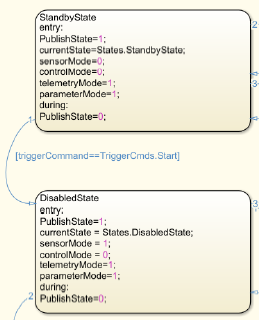
\includegraphics[width=1.79167in]{jira_imgs/1019.png}\\
If the configuration file is invalid or out of range, the system will
transition into a Fault State

\medskip }
\end{minipage} \\ \cdashline{2-2}

 & Actual Result \\
 & \begin{minipage}[t]{15cm}{\footnotesize
\smallskip

\medskip }
\end{minipage} \\ \cdashline{2-2}

 & Status: \textbf{ Not Executed } \\ \hline

7 & Description \\
 & \begin{minipage}[t]{15cm}
{\footnotesize
\smallskip
\textbf{DISABLEDSTATE -\textgreater{} ENABLEDSTATE}\\
From the DisabledState, send an enable state command through the DDS.\\
\textbf{}

\medskip }
\end{minipage}
\\ \cdashline{2-2}


 & Expected Result \\
 & \begin{minipage}[t]{15cm}{\footnotesize
\smallskip
The system transitions into the EnabledState/Stationary substate, the
motor drives are enabled, motor brakes are released and the system is
capable of receiving/responding to DDS commands.\\
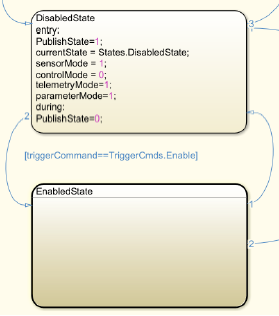
\includegraphics[width=1.79167in]{jira_imgs/1020.png}\\

\medskip }
\end{minipage} \\ \cdashline{2-2}

 & Actual Result \\
 & \begin{minipage}[t]{15cm}{\footnotesize
\smallskip

\medskip }
\end{minipage} \\ \cdashline{2-2}

 & Status: \textbf{ Not Executed } \\ \hline

8 & Description \\
 & \begin{minipage}[t]{15cm}
{\footnotesize
\smallskip
\textbf{FAULTSTATE}\\
If a Fault occurs in any of the other states, the system will
automatically transition to the Fault State. While in the Fault state,
send a clearError command through the DDS.\\
Note: If the fault that occurs goes through the interlock system, reset
the safety relay switch and send a clearError command.

\medskip }
\end{minipage}
\\ \cdashline{2-2}


 & Expected Result \\
 & \begin{minipage}[t]{15cm}{\footnotesize
\smallskip
The system transitions back to the OfflineState/PublishOnly substate and
is not capable of receiving/responding to DDS commands. (Go back to Step
3)\\
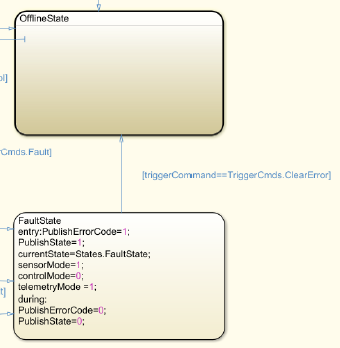
\includegraphics[width=1.79167in]{jira_imgs/1021.png}

\medskip }
\end{minipage} \\ \cdashline{2-2}

 & Actual Result \\
 & \begin{minipage}[t]{15cm}{\footnotesize
\smallskip

\medskip }
\end{minipage} \\ \cdashline{2-2}

 & Status: \textbf{ Not Executed } \\ \hline

9 & Description \\
 & \begin{minipage}[t]{15cm}
{\footnotesize
\smallskip
Start up the CCW such that it is in the Enabled state. \textbf{{(Need
details from Tekniker)}}

\medskip }
\end{minipage}
\\ \cdashline{2-2}


 & Expected Result \\
 & \begin{minipage}[t]{15cm}{\footnotesize
\smallskip

\medskip }
\end{minipage} \\ \cdashline{2-2}

 & Actual Result \\
 & \begin{minipage}[t]{15cm}{\footnotesize
\smallskip

\medskip }
\end{minipage} \\ \cdashline{2-2}

 & Status: \textbf{ Not Executed } \\ \hline

10 & Description \\
 & \begin{minipage}[t]{15cm}
{\footnotesize
\smallskip
\textbf{Camera Rotator Interlock}\\[2\baselineskip]With the CCW and the
Camera Rotator in the Enabled state, but \textbf{NOT} moving, unlock and
rotate the rotator locking pin such that it is no longer depressing the
fully retracted limit switches.\\
{\\
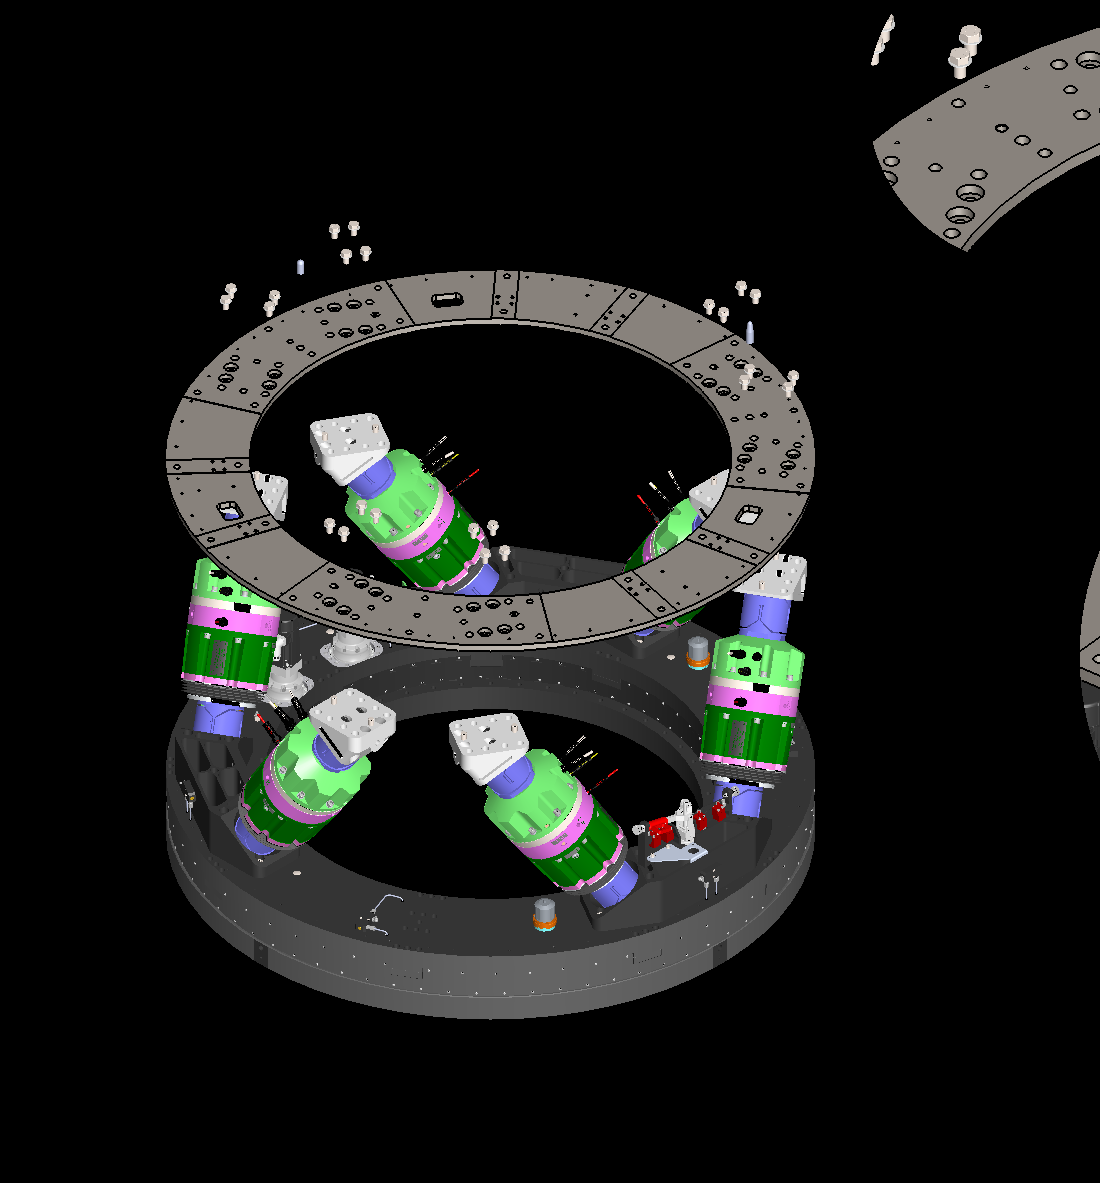
\includegraphics[width=3.12500in]{jira_imgs/998.png}}\\
{\\
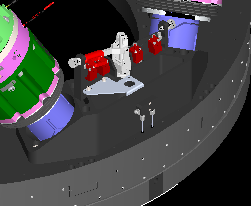
\includegraphics[width=3.12500in]{jira_imgs/999.png}}

\medskip }
\end{minipage}
\\ \cdashline{2-2}


 & Expected Result \\
 & \begin{minipage}[t]{15cm}{\footnotesize
\smallskip
The fault within the Camera Rotator Interlock System disables the Camera
Rotator and CCW drives by a Safe Torque Off trigger.

\medskip }
\end{minipage} \\ \cdashline{2-2}

 & Actual Result \\
 & \begin{minipage}[t]{15cm}{\footnotesize
\smallskip

\medskip }
\end{minipage} \\ \cdashline{2-2}

 & Status: \textbf{ Not Executed } \\ \hline

11 & Description \\
 & \begin{minipage}[t]{15cm}
{\footnotesize
\smallskip
Manually reset the interlock system by cycling the safety reset switch.

\medskip }
\end{minipage}
\\ \cdashline{2-2}


 & Expected Result \\
 & \begin{minipage}[t]{15cm}{\footnotesize
\smallskip
The safety interlock fault has been cleared in the PILZ controller.

\medskip }
\end{minipage} \\ \cdashline{2-2}

 & Actual Result \\
 & \begin{minipage}[t]{15cm}{\footnotesize
\smallskip

\medskip }
\end{minipage} \\ \cdashline{2-2}

 & Status: \textbf{ Not Executed } \\ \hline

12 & Description \\
 & \begin{minipage}[t]{15cm}
{\footnotesize
\smallskip
Transition out of the fault state by sending a ClearError trigger.

\medskip }
\end{minipage}
\\ \cdashline{2-2}


 & Expected Result \\
 & \begin{minipage}[t]{15cm}{\footnotesize
\smallskip
The system transitions from the Fault state to the Offline/PublishOnly
State.

\medskip }
\end{minipage} \\ \cdashline{2-2}

 & Actual Result \\
 & \begin{minipage}[t]{15cm}{\footnotesize
\smallskip

\medskip }
\end{minipage} \\ \cdashline{2-2}

 & Status: \textbf{ Not Executed } \\ \hline

13 & Description \\
 & \begin{minipage}[t]{15cm}
{\footnotesize
\smallskip
Bring the CCW and the Camera Rotator back to the Enabled state.

\medskip }
\end{minipage}
\\ \cdashline{2-2}


 & Expected Result \\
 & \begin{minipage}[t]{15cm}{\footnotesize
\smallskip
CCW and Camera Rotator are in the Enabled state.

\medskip }
\end{minipage} \\ \cdashline{2-2}

 & Actual Result \\
 & \begin{minipage}[t]{15cm}{\footnotesize
\smallskip

\medskip }
\end{minipage} \\ \cdashline{2-2}

 & Status: \textbf{ Not Executed } \\ \hline

14 & Description \\
 & \begin{minipage}[t]{15cm}
{\footnotesize
\smallskip
\textbf{CCW Interlock}\\
\textbf{{(Need details from Tekniker)}}

\medskip }
\end{minipage}
\\ \cdashline{2-2}


 & Expected Result \\
 & \begin{minipage}[t]{15cm}{\footnotesize
\smallskip
The fault within the CCW AUX Interlock System disables the Camera
Rotator and CCW drives by a Safe Torque Off function.

\medskip }
\end{minipage} \\ \cdashline{2-2}

 & Actual Result \\
 & \begin{minipage}[t]{15cm}{\footnotesize
\smallskip

\medskip }
\end{minipage} \\ \cdashline{2-2}

 & Status: \textbf{ Not Executed } \\ \hline

15 & Description \\
 & \begin{minipage}[t]{15cm}
{\footnotesize
\smallskip
Bring the CCW and the Camera Rotator back to the Enabled state.

\medskip }
\end{minipage}
\\ \cdashline{2-2}


 & Expected Result \\
 & \begin{minipage}[t]{15cm}{\footnotesize
\smallskip
CCW and Camera Rotator are in the Enabled state.

\medskip }
\end{minipage} \\ \cdashline{2-2}

 & Actual Result \\
 & \begin{minipage}[t]{15cm}{\footnotesize
\smallskip

\medskip }
\end{minipage} \\ \cdashline{2-2}

 & Status: \textbf{ Not Executed } \\ \hline

16 & Description \\
 & \begin{minipage}[t]{15cm}
{\footnotesize
\smallskip
{\textbf{Manual Test of the CCW Interlock}\\[2\baselineskip]Remove the
locking pin from the bar connecting the CCW and the Camera Rotator.}

\medskip }
\end{minipage}
\\ \cdashline{2-2}


 & Expected Result \\
 & \begin{minipage}[t]{15cm}{\footnotesize
\smallskip
{The CCW is able to move independently. }

\medskip }
\end{minipage} \\ \cdashline{2-2}

 & Actual Result \\
 & \begin{minipage}[t]{15cm}{\footnotesize
\smallskip

\medskip }
\end{minipage} \\ \cdashline{2-2}

 & Status: \textbf{ Not Executed } \\ \hline

17 & Description \\
 & \begin{minipage}[t]{15cm}
{\footnotesize
\smallskip
{Manually twist the bar connected to the CCW in the positive direction
until the positive limit switch is tripped.}

\medskip }
\end{minipage}
\\ \cdashline{2-2}


 & Expected Result \\
 & \begin{minipage}[t]{15cm}{\footnotesize
\smallskip
{The fault triggered on the CCW positive limit switch disables drives
for both the CCW and the Camera Rotator by a Safe Torque Off trigger.}

\medskip }
\end{minipage} \\ \cdashline{2-2}

 & Actual Result \\
 & \begin{minipage}[t]{15cm}{\footnotesize
\smallskip

\medskip }
\end{minipage} \\ \cdashline{2-2}

 & Status: \textbf{ Not Executed } \\ \hline

18 & Description \\
 & \begin{minipage}[t]{15cm}
{\footnotesize
\smallskip
Rotate the bar so that it is approximately at 0 degrees.

\medskip }
\end{minipage}
\\ \cdashline{2-2}


 & Expected Result \\
 & \begin{minipage}[t]{15cm}{\footnotesize
\smallskip
The CCW is midway between the limit switches.

\medskip }
\end{minipage} \\ \cdashline{2-2}

 & Actual Result \\
 & \begin{minipage}[t]{15cm}{\footnotesize
\smallskip

\medskip }
\end{minipage} \\ \cdashline{2-2}

 & Status: \textbf{ Not Executed } \\ \hline

19 & Description \\
 & \begin{minipage}[t]{15cm}
{\footnotesize
\smallskip
{Reset the interlock for the CCW (Tekniker) and Camera Rotator (see step
1.8 above)}

\medskip }
\end{minipage}
\\ \cdashline{2-2}


 & Expected Result \\
 & \begin{minipage}[t]{15cm}{\footnotesize
\smallskip
{The CCW and Camera Rotator are in the Enabled State.}

\medskip }
\end{minipage} \\ \cdashline{2-2}

 & Actual Result \\
 & \begin{minipage}[t]{15cm}{\footnotesize
\smallskip

\medskip }
\end{minipage} \\ \cdashline{2-2}

 & Status: \textbf{ Not Executed } \\ \hline

20 & Description \\
 & \begin{minipage}[t]{15cm}
{\footnotesize
\smallskip
{Manually twist the bar connected to the CCW in the negative direction
until the interlock is tripped.}

\medskip }
\end{minipage}
\\ \cdashline{2-2}


 & Expected Result \\
 & \begin{minipage}[t]{15cm}{\footnotesize
\smallskip
{The fault triggered on the CCW negative limit switch disables the
drives on the CCW by a Safe Torque Off Trigger.\\
}

\medskip }
\end{minipage} \\ \cdashline{2-2}

 & Actual Result \\
 & \begin{minipage}[t]{15cm}{\footnotesize
\smallskip

\medskip }
\end{minipage} \\ \cdashline{2-2}

 & Status: \textbf{ Not Executed } \\ \hline

21 & Description \\
 & \begin{minipage}[t]{15cm}
{\footnotesize
\smallskip
Rotate the bar so that it is approximately at 0 degrees.

\medskip }
\end{minipage}
\\ \cdashline{2-2}


 & Expected Result \\
 & \begin{minipage}[t]{15cm}{\footnotesize
\smallskip
The CCW is midway between the limit switches.

\medskip }
\end{minipage} \\ \cdashline{2-2}

 & Actual Result \\
 & \begin{minipage}[t]{15cm}{\footnotesize
\smallskip

\medskip }
\end{minipage} \\ \cdashline{2-2}

 & Status: \textbf{ Not Executed } \\ \hline

22 & Description \\
 & \begin{minipage}[t]{15cm}
{\footnotesize
\smallskip
Reset the interlock for the CCW (Tekniker) and Camera Rotator (see step
1.8 above)

\medskip }
\end{minipage}
\\ \cdashline{2-2}


 & Expected Result \\
 & \begin{minipage}[t]{15cm}{\footnotesize
\smallskip
The CCW and Camera Rotator are in the Enabled State.

\medskip }
\end{minipage} \\ \cdashline{2-2}

 & Actual Result \\
 & \begin{minipage}[t]{15cm}{\footnotesize
\smallskip

\medskip }
\end{minipage} \\ \cdashline{2-2}

 & Status: \textbf{ Not Executed } \\ \hline

23 & Description \\
 & \begin{minipage}[t]{15cm}
{\footnotesize
\smallskip
{Remove the locking pin that so that the CCW moves independently from
the CR.}

\medskip }
\end{minipage}
\\ \cdashline{2-2}


 & Expected Result \\
 & \begin{minipage}[t]{15cm}{\footnotesize
\smallskip

\medskip }
\end{minipage} \\ \cdashline{2-2}

 & Actual Result \\
 & \begin{minipage}[t]{15cm}{\footnotesize
\smallskip

\medskip }
\end{minipage} \\ \cdashline{2-2}

 & Status: \textbf{ Not Executed } \\ \hline

24 & Description \\
 & \begin{minipage}[t]{15cm}
{\footnotesize
\smallskip
The following steps define what the Jupyter Notebook for this test case
implements. Executing the Jupyter notebook is the only actual step that
needs to be executed.

\medskip }
\end{minipage}
\\ \cdashline{2-2}


 & Expected Result \\
 & \begin{minipage}[t]{15cm}{\footnotesize
\smallskip

\medskip }
\end{minipage} \\ \cdashline{2-2}

 & Actual Result \\
 & \begin{minipage}[t]{15cm}{\footnotesize
\smallskip

\medskip }
\end{minipage} \\ \cdashline{2-2}

 & Status: \textbf{ Not Executed } \\ \hline

25 & Description \\
 & \begin{minipage}[t]{15cm}
{\footnotesize
\smallskip
Send a trackStart command to the rotator.~

\medskip }
\end{minipage}
\\ \cdashline{2-2}


 & Expected Result \\
 & \begin{minipage}[t]{15cm}{\footnotesize
\smallskip

\medskip }
\end{minipage} \\ \cdashline{2-2}

 & Actual Result \\
 & \begin{minipage}[t]{15cm}{\footnotesize
\smallskip

\medskip }
\end{minipage} \\ \cdashline{2-2}

 & Status: \textbf{ Not Executed } \\ \hline

26 & Description \\
 & \begin{minipage}[t]{15cm}
{\footnotesize
\smallskip
Send a track command via the pointing component to track in the positive
direction.

\medskip }
\end{minipage}
\\ \cdashline{2-2}


 & Expected Result \\
 & \begin{minipage}[t]{15cm}{\footnotesize
\smallskip

\medskip }
\end{minipage} \\ \cdashline{2-2}

 & Actual Result \\
 & \begin{minipage}[t]{15cm}{\footnotesize
\smallskip

\medskip }
\end{minipage} \\ \cdashline{2-2}

 & Status: \textbf{ Not Executed } \\ \hline

27 & Description \\
 & \begin{minipage}[t]{15cm}
{\footnotesize
\smallskip
{Using the encoders, verify that the CCW and CR are moving
synchronously. (}{If we run the test asynchronously, we just need to
check the CCW and CR are within the 2.2 degrees of each other}{)}

\medskip }
\end{minipage}
\\ \cdashline{2-2}


 & Expected Result \\
 & \begin{minipage}[t]{15cm}{\footnotesize
\smallskip

\medskip }
\end{minipage} \\ \cdashline{2-2}

 & Actual Result \\
 & \begin{minipage}[t]{15cm}{\footnotesize
\smallskip

\medskip }
\end{minipage} \\ \cdashline{2-2}

 & Status: \textbf{ Not Executed } \\ \hline

28 & Description \\
 & \begin{minipage}[t]{15cm}
{\footnotesize
\smallskip
{\textbf{WOBBLE Interlock~}\\[2\baselineskip]Reinsert the locking pin
for the bar connecting the CCW and Camera Rotator}

\medskip }
\end{minipage}
\\ \cdashline{2-2}


 & Expected Result \\
 & \begin{minipage}[t]{15cm}{\footnotesize
\smallskip
{The CCW and Camera Rotator are both mechanically and electrically
connected. }\\[2\baselineskip]

\medskip }
\end{minipage} \\ \cdashline{2-2}

 & Actual Result \\
 & \begin{minipage}[t]{15cm}{\footnotesize
\smallskip

\medskip }
\end{minipage} \\ \cdashline{2-2}

 & Status: \textbf{ Not Executed } \\ \hline

29 & Description \\
 & \begin{minipage}[t]{15cm}
{\footnotesize
\smallskip
{With the Camera Rotator in the enabled/stationary state and both the
Camera Rotator and CCW not moving, send a positionSet command of 0
degrees.}

\medskip }
\end{minipage}
\\ \cdashline{2-2}


 & Expected Result \\
 & \begin{minipage}[t]{15cm}{\footnotesize
\smallskip
{The Camera Rotator and the CCW do not move.}

\medskip }
\end{minipage} \\ \cdashline{2-2}

 & Actual Result \\
 & \begin{minipage}[t]{15cm}{\footnotesize
\smallskip

\medskip }
\end{minipage} \\ \cdashline{2-2}

 & Status: \textbf{ Not Executed } \\ \hline

30 & Description \\
 & \begin{minipage}[t]{15cm}
{\footnotesize
\smallskip
{Send a move command}

\medskip }
\end{minipage}
\\ \cdashline{2-2}


 & Expected Result \\
 & \begin{minipage}[t]{15cm}{\footnotesize
\smallskip
{The Camera Rotator and the CCW are at 0 degrees.}

\medskip }
\end{minipage} \\ \cdashline{2-2}

 & Actual Result \\
 & \begin{minipage}[t]{15cm}{\footnotesize
\smallskip

\medskip }
\end{minipage} \\ \cdashline{2-2}

 & Status: \textbf{ Not Executed } \\ \hline

31 & Description \\
 & \begin{minipage}[t]{15cm}
{\footnotesize
\smallskip
{Send a velocitySet command of +0.1\textbf{~}deg/s and 23 seconds.
}{\\[2\baselineskip]}

\medskip }
\end{minipage}
\\ \cdashline{2-2}


 & Expected Result \\
 & \begin{minipage}[t]{15cm}{\footnotesize
\smallskip
{The Camera Rotator and CCW do not move.}

\medskip }
\end{minipage} \\ \cdashline{2-2}

 & Actual Result \\
 & \begin{minipage}[t]{15cm}{\footnotesize
\smallskip

\medskip }
\end{minipage} \\ \cdashline{2-2}

 & Status: \textbf{ Not Executed } \\ \hline

32 & Description \\
 & \begin{minipage}[t]{15cm}
{\footnotesize
\smallskip
{Send a moveConstantVelocity command}

\medskip }
\end{minipage}
\\ \cdashline{2-2}


 & Expected Result \\
 & \begin{minipage}[t]{15cm}{\footnotesize
\smallskip
{The Camera Rotator begins to move while the CCW remains idle.}

\medskip }
\end{minipage} \\ \cdashline{2-2}

 & Actual Result \\
 & \begin{minipage}[t]{15cm}{\footnotesize
\smallskip

\medskip }
\end{minipage} \\ \cdashline{2-2}

 & Status: \textbf{ Not Executed } \\ \hline

33 & Description \\
 & \begin{minipage}[t]{15cm}
{\footnotesize
\smallskip
{Verify the positive limit switch is tripped on the wobble assembly.}\\
{\\
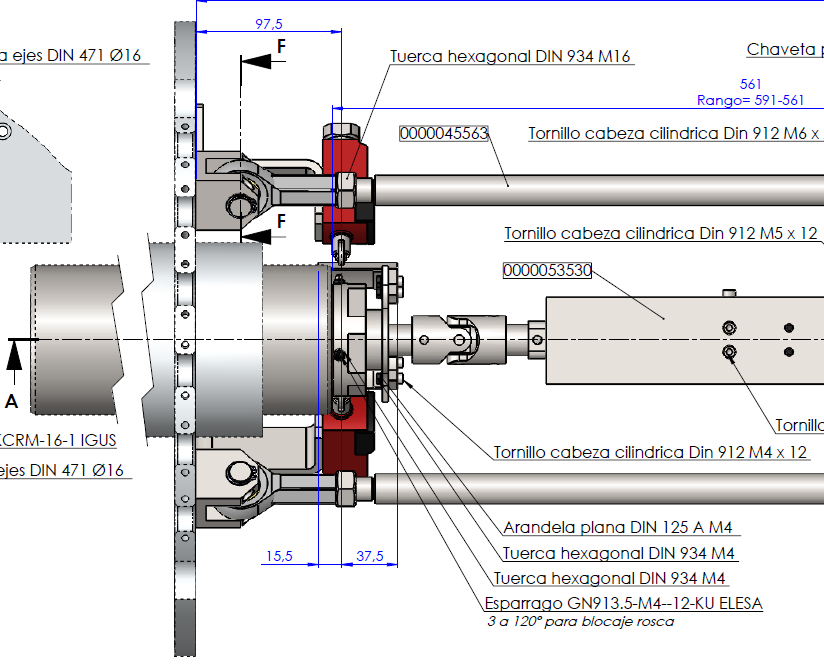
\includegraphics[width=3.12500in]{jira_imgs/1032.png}~}

\medskip }
\end{minipage}
\\ \cdashline{2-2}


 & Expected Result \\
 & \begin{minipage}[t]{15cm}{\footnotesize
\smallskip
{The fault triggered on the WOBBLE positive limit switch disables the
drives on both the Camera Rotator and CCW drives by a Safe Torque Off
trigger.}

\medskip }
\end{minipage} \\ \cdashline{2-2}

 & Actual Result \\
 & \begin{minipage}[t]{15cm}{\footnotesize
\smallskip

\medskip }
\end{minipage} \\ \cdashline{2-2}

 & Status: \textbf{ Not Executed } \\ \hline

34 & Description \\
 & \begin{minipage}[t]{15cm}
{\footnotesize
\smallskip
Verify the location of the positive limit switch is equal to or less
than 2.2 degrees.

\medskip }
\end{minipage}
\\ \cdashline{2-2}


 & Expected Result \\
 & \begin{minipage}[t]{15cm}{\footnotesize
\smallskip
The Camera Rotator is within 2.2 degrees of the CCW.~

\medskip }
\end{minipage} \\ \cdashline{2-2}

 & Actual Result \\
 & \begin{minipage}[t]{15cm}{\footnotesize
\smallskip

\medskip }
\end{minipage} \\ \cdashline{2-2}

 & Status: \textbf{ Not Executed } \\ \hline

35 & Description \\
 & \begin{minipage}[t]{15cm}
{\footnotesize
\smallskip
Reset the wobble interlock.

\medskip }
\end{minipage}
\\ \cdashline{2-2}


 & Expected Result \\
 & \begin{minipage}[t]{15cm}{\footnotesize
\smallskip
{The Camera Rotator and CCW drives are both on and are in the Enabled
State.}

\medskip }
\end{minipage} \\ \cdashline{2-2}

 & Actual Result \\
 & \begin{minipage}[t]{15cm}{\footnotesize
\smallskip

\medskip }
\end{minipage} \\ \cdashline{2-2}

 & Status: \textbf{ Not Executed } \\ \hline

36 & Description \\
 & \begin{minipage}[t]{15cm}
{\footnotesize
\smallskip
{With the Camera Rotator in the enabled/stationary state and both the
Camera Rotator and CCW not moving, send a positionSet command of 0
degrees.}

\medskip }
\end{minipage}
\\ \cdashline{2-2}


 & Expected Result \\
 & \begin{minipage}[t]{15cm}{\footnotesize
\smallskip
{The Camera Rotator and the CCW do not move.}

\medskip }
\end{minipage} \\ \cdashline{2-2}

 & Actual Result \\
 & \begin{minipage}[t]{15cm}{\footnotesize
\smallskip

\medskip }
\end{minipage} \\ \cdashline{2-2}

 & Status: \textbf{ Not Executed } \\ \hline

37 & Description \\
 & \begin{minipage}[t]{15cm}
{\footnotesize
\smallskip
{Send a move command.}

\medskip }
\end{minipage}
\\ \cdashline{2-2}


 & Expected Result \\
 & \begin{minipage}[t]{15cm}{\footnotesize
\smallskip
{The Camera Rotator moves back to exactly 0 degrees and the CCW does not
move.}

\medskip }
\end{minipage} \\ \cdashline{2-2}

 & Actual Result \\
 & \begin{minipage}[t]{15cm}{\footnotesize
\smallskip

\medskip }
\end{minipage} \\ \cdashline{2-2}

 & Status: \textbf{ Not Executed } \\ \hline

38 & Description \\
 & \begin{minipage}[t]{15cm}
{\footnotesize
\smallskip
{Send a velocitySet command of -0.1\textbf{~}deg/s and 23 seconds.~\\
}{\\
}

\medskip }
\end{minipage}
\\ \cdashline{2-2}


 & Expected Result \\
 & \begin{minipage}[t]{15cm}{\footnotesize
\smallskip
{The Camera Rotator and CCW do not move.}

\medskip }
\end{minipage} \\ \cdashline{2-2}

 & Actual Result \\
 & \begin{minipage}[t]{15cm}{\footnotesize
\smallskip

\medskip }
\end{minipage} \\ \cdashline{2-2}

 & Status: \textbf{ Not Executed } \\ \hline

39 & Description \\
 & \begin{minipage}[t]{15cm}
{\footnotesize
\smallskip
{Send a moveConstantVelocity command}

\medskip }
\end{minipage}
\\ \cdashline{2-2}


 & Expected Result \\
 & \begin{minipage}[t]{15cm}{\footnotesize
\smallskip
{The Camera Rotator begins to move while the CCW remains idle.}

\medskip }
\end{minipage} \\ \cdashline{2-2}

 & Actual Result \\
 & \begin{minipage}[t]{15cm}{\footnotesize
\smallskip

\medskip }
\end{minipage} \\ \cdashline{2-2}

 & Status: \textbf{ Not Executed } \\ \hline

40 & Description \\
 & \begin{minipage}[t]{15cm}
{\footnotesize
\smallskip
{Verify the negative limit switch is tripped on the wobble assembly.}\\
{\\
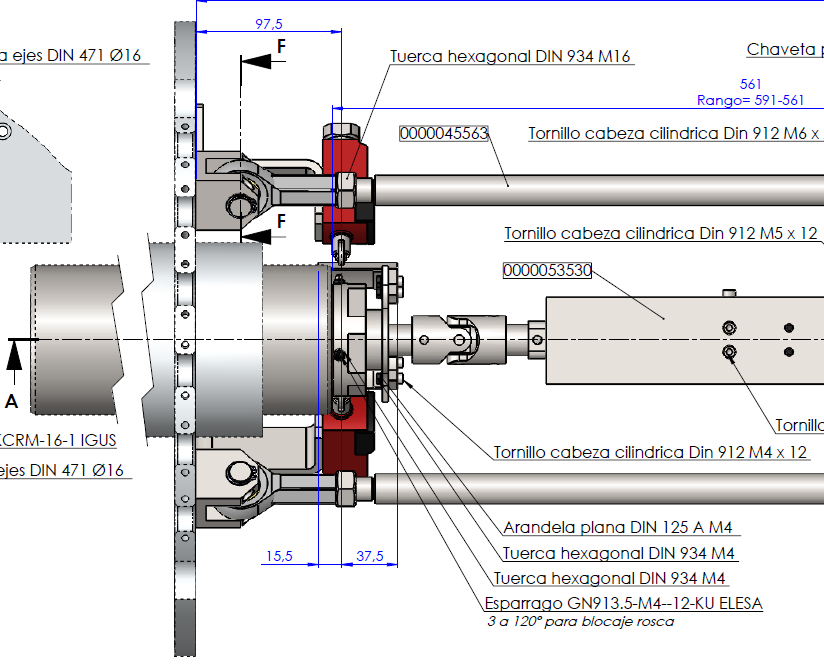
\includegraphics[width=3.12500in]{jira_imgs/1032.png}~}

\medskip }
\end{minipage}
\\ \cdashline{2-2}


 & Expected Result \\
 & \begin{minipage}[t]{15cm}{\footnotesize
\smallskip
{The fault triggered on the WOBBLE negative limit switch disables the
drives on both the Camera Rotator and CCW drives by a Safe Torque Off
trigger.}

\medskip }
\end{minipage} \\ \cdashline{2-2}

 & Actual Result \\
 & \begin{minipage}[t]{15cm}{\footnotesize
\smallskip

\medskip }
\end{minipage} \\ \cdashline{2-2}

 & Status: \textbf{ Not Executed } \\ \hline

41 & Description \\
 & \begin{minipage}[t]{15cm}
{\footnotesize
\smallskip
Verify the location of the negative limit switch is equal to or less
than 2.2 degrees.

\medskip }
\end{minipage}
\\ \cdashline{2-2}


 & Expected Result \\
 & \begin{minipage}[t]{15cm}{\footnotesize
\smallskip

\medskip }
\end{minipage} \\ \cdashline{2-2}

 & Actual Result \\
 & \begin{minipage}[t]{15cm}{\footnotesize
\smallskip

\medskip }
\end{minipage} \\ \cdashline{2-2}

 & Status: \textbf{ Not Executed } \\ \hline

42 & Description \\
 & \begin{minipage}[t]{15cm}
{\footnotesize
\smallskip
Reset the wobble interlock.

\medskip }
\end{minipage}
\\ \cdashline{2-2}


 & Expected Result \\
 & \begin{minipage}[t]{15cm}{\footnotesize
\smallskip
{The Camera Rotator and CCW drives are both on and are in the Enabled
State.}

\medskip }
\end{minipage} \\ \cdashline{2-2}

 & Actual Result \\
 & \begin{minipage}[t]{15cm}{\footnotesize
\smallskip

\medskip }
\end{minipage} \\ \cdashline{2-2}

 & Status: \textbf{ Not Executed } \\ \hline

43 & Description \\
 & \begin{minipage}[t]{15cm}
{\footnotesize
\smallskip
{With the Camera Rotator in the enabled/stationary state and both the
Camera Rotator and CCW not moving, send a positionSet command of 0
degrees.}

\medskip }
\end{minipage}
\\ \cdashline{2-2}


 & Expected Result \\
 & \begin{minipage}[t]{15cm}{\footnotesize
\smallskip
{The Camera Rotator and the CCW do not move.}

\medskip }
\end{minipage} \\ \cdashline{2-2}

 & Actual Result \\
 & \begin{minipage}[t]{15cm}{\footnotesize
\smallskip

\medskip }
\end{minipage} \\ \cdashline{2-2}

 & Status: \textbf{ Not Executed } \\ \hline

44 & Description \\
 & \begin{minipage}[t]{15cm}
{\footnotesize
\smallskip
{Send a moveConstantVelocity command}

\medskip }
\end{minipage}
\\ \cdashline{2-2}


 & Expected Result \\
 & \begin{minipage}[t]{15cm}{\footnotesize
\smallskip
{The Camera Rotator begins to move while the CCW remains idle.}

\medskip }
\end{minipage} \\ \cdashline{2-2}

 & Actual Result \\
 & \begin{minipage}[t]{15cm}{\footnotesize
\smallskip

\medskip }
\end{minipage} \\ \cdashline{2-2}

 & Status: \textbf{ Not Executed } \\ \hline

45 & Description \\
 & \begin{minipage}[t]{15cm}
{\footnotesize
\smallskip
\textbf{{E-Stop Test (Move the Camera Rotator and CCW at full speed, hit
the E-Stop and verify that they are stopped at the same degree)}}

\medskip }
\end{minipage}
\\ \cdashline{2-2}


 & Expected Result \\
 & \begin{minipage}[t]{15cm}{\footnotesize
\smallskip

\medskip }
\end{minipage} \\ \cdashline{2-2}

 & Actual Result \\
 & \begin{minipage}[t]{15cm}{\footnotesize
\smallskip

\medskip }
\end{minipage} \\ \cdashline{2-2}

 & Status: \textbf{ Not Executed } \\ \hline

46 & Description \\
 & \begin{minipage}[t]{15cm}
{\footnotesize
\smallskip

\medskip }
\end{minipage}
\\ \cdashline{2-2}


 & Expected Result \\
 & \begin{minipage}[t]{15cm}{\footnotesize
\smallskip

\medskip }
\end{minipage} \\ \cdashline{2-2}

 & Actual Result \\
 & \begin{minipage}[t]{15cm}{\footnotesize
\smallskip

\medskip }
\end{minipage} \\ \cdashline{2-2}

 & Status: \textbf{ Not Executed } \\ \hline

47 & Description \\
 & \begin{minipage}[t]{15cm}
{\footnotesize
\smallskip

\medskip }
\end{minipage}
\\ \cdashline{2-2}


 & Expected Result \\
 & \begin{minipage}[t]{15cm}{\footnotesize
\smallskip

\medskip }
\end{minipage} \\ \cdashline{2-2}

 & Actual Result \\
 & \begin{minipage}[t]{15cm}{\footnotesize
\smallskip

\medskip }
\end{minipage} \\ \cdashline{2-2}

 & Status: \textbf{ Not Executed } \\ \hline

48 & Description \\
 & \begin{minipage}[t]{15cm}
{\footnotesize
\smallskip
Shutdown the CCW and Camera Rotator.

\medskip }
\end{minipage}
\\ \cdashline{2-2}


 & Expected Result \\
 & \begin{minipage}[t]{15cm}{\footnotesize
\smallskip
The CCW and Camera Rotator are shutdown.

\medskip }
\end{minipage} \\ \cdashline{2-2}

 & Actual Result \\
 & \begin{minipage}[t]{15cm}{\footnotesize
\smallskip

\medskip }
\end{minipage} \\ \cdashline{2-2}

 & Status: \textbf{ Not Executed } \\ \hline

\end{longtable}

\paragraph{Test Case LVV-T1588 - Pointing Component Control Test
 }\mbox{}\\

Open  \href{https://jira.lsstcorp.org/secure/Tests.jspa#/testCase/LVV-T1588}{\textit{ LVV-T1588 } }
test case in Jira.

The objective of this test case is to verify the combined control of the
integrated CCW and Camera Rotator via the LSST pointing component as
specified in \citeds{LTS-218}. This test case will exercise the functionality of
the synchronized CCW and Camera Rotator during tracking and move
commands and meeting the following criteria:

\begin{itemize}
\tightlist
\item
  Does \textbf{NOT} require the Camera Rotator to be loaded with the
  camera simulated mass or actual camera hardware
\end{itemize}

This test case will execute 4 scenarios:

\begin{enumerate}
\tightlist
\item
  Basic Control Scenario
\item
  High Rotation Stress Test Scenario

  \begin{itemize}
  \tightlist
  \item
    Full operational range of motion from +90 to -90
  \end{itemize}
\item
  Filter Change Scenario
\item
  Typical Night

  \begin{itemize}
  \tightlist
  \item
    Verify the CCW does not rotate during exposure
  \item
    Execute an extended exposure
  \end{itemize}
\end{enumerate}


\textbf{ Preconditions}:\\
Prior to the execution of this test case to verify the pointing
component of the CCW + Camera Rotator, the following Summit tasks must
be completed:

\begin{itemize}
\tightlist
\item
  The CCW has been installed on the Camera Cart

  \begin{itemize}
  \tightlist
  \item
    \url{https://jira.lsstcorp.org/browse/SUMMIT-2156}
  \end{itemize}
\item
  The Camera Hexapod/Rotator Controller has been deployed on the summit

  \begin{itemize}
  \tightlist
  \item
    \url{https://jira.lsstcorp.org/browse/SUMMIT-3229}
  \end{itemize}
\item
  The Combined Motion of the CCW + Rotator has been verified to be in
  sync

  \begin{itemize}
  \tightlist
  \item
    \url{https://jira.lsstcorp.org/browse/SUMMIT-3295}
  \end{itemize}
\end{itemize}


Execution status: {\bf Not Executed }

Final comment:\\


Detailed steps results:

\begin{longtable}{p{1cm}p{15cm}}
\hline
{Step} & Step Details\\ \hline
1 & Description \\
 & \begin{minipage}[t]{15cm}
{\footnotesize
\smallskip
\textbf{STARTING THE EUI}\\[2\baselineskip]Double click the Hexapod GUI
Viewer desktop icon on the computer.

\begin{itemize}
\tightlist
\item
  This can be done on the Dell Management PC or another computer on the
  same network
\end{itemize}

\medskip }
\end{minipage}
\\ \cdashline{2-2}


 & Expected Result \\
 & \begin{minipage}[t]{15cm}{\footnotesize
\smallskip
A prompt to enter a password is shown.~

\medskip }
\end{minipage} \\ \cdashline{2-2}

 & Actual Result \\
 & \begin{minipage}[t]{15cm}{\footnotesize
\smallskip

\medskip }
\end{minipage} \\ \cdashline{2-2}

 & Status: \textbf{ Not Executed } \\ \hline

2 & Description \\
 & \begin{minipage}[t]{15cm}
{\footnotesize
\smallskip
Enter the password ``lsst-vnc''

\begin{itemize}
\tightlist
\item
  If the EUI isn't automatically up and running when the VNC opens,
  double click on the CAM\_Hex\_eGUI or M2\_Hex\_eGUI icon on the VNC
  viewer
\end{itemize}

\medskip }
\end{minipage}
\\ \cdashline{2-2}


 & Expected Result \\
 & \begin{minipage}[t]{15cm}{\footnotesize
\smallskip
The EUI is in the Offline State/PublishOnly substate and is able to
publish through SAL but cannot receive commands.

\medskip }
\end{minipage} \\ \cdashline{2-2}

 & Actual Result \\
 & \begin{minipage}[t]{15cm}{\footnotesize
\smallskip

\medskip }
\end{minipage} \\ \cdashline{2-2}

 & Status: \textbf{ Not Executed } \\ \hline

3 & Description \\
 & \begin{minipage}[t]{15cm}
{\footnotesize
\smallskip
\textbf{OFFLINESTATE/AVAILABLESTATE}\\
On the Main tab, select the ``Offline SubState Cmd'' field in the
Commands to Send section, set the Offline SubState Triggers to ``System
Ready'' and click on the Send Command button.\\
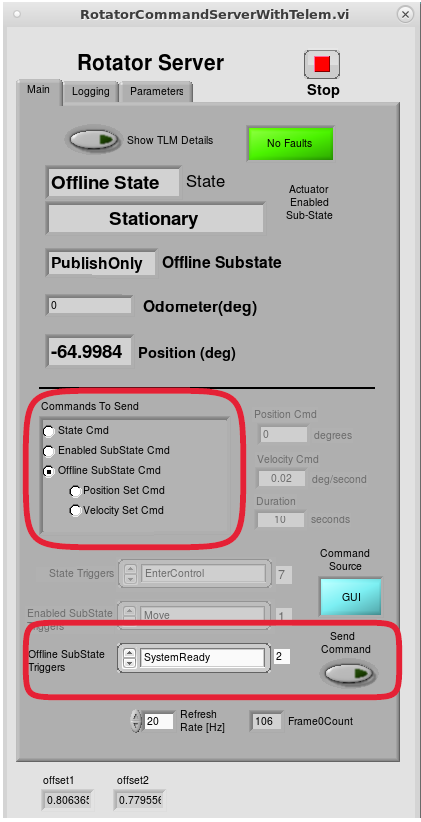
\includegraphics[width=1.79167in]{jira_imgs/1005.png}

\medskip }
\end{minipage}
\\ \cdashline{2-2}


 & Expected Result \\
 & \begin{minipage}[t]{15cm}{\footnotesize
\smallskip
The system transitions from the OfflineState/PublishOnly substate to the
OfflineState/AvailableState
substate.\\[2\baselineskip]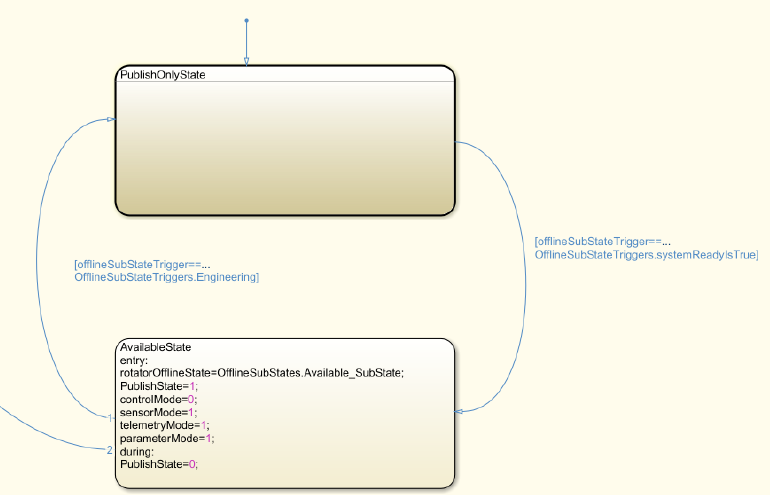
\includegraphics[width=1.79167in]{jira_imgs/1007.png}

\medskip }
\end{minipage} \\ \cdashline{2-2}

 & Actual Result \\
 & \begin{minipage}[t]{15cm}{\footnotesize
\smallskip

\medskip }
\end{minipage} \\ \cdashline{2-2}

 & Status: \textbf{ Not Executed } \\ \hline

4 & Description \\
 & \begin{minipage}[t]{15cm}
{\footnotesize
\smallskip
\textbf{SWITCHING TO DDS MODE}\\
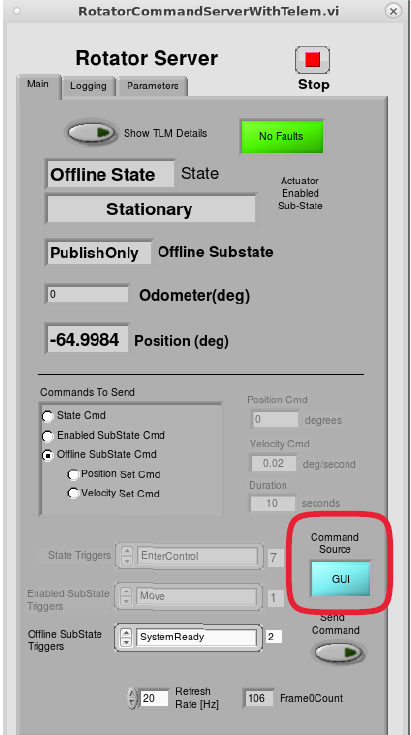
\includegraphics[width=1.79167in]{jira_imgs/1014.png}\\
If the Command Source does not show DDS, go to the Parameters tab,
select DDS under the Command Source and click the Set Command Source
button.\\
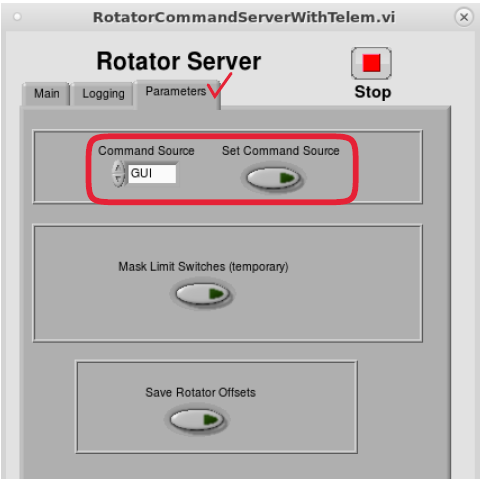
\includegraphics[width=1.79167in]{jira_imgs/1013.png}\textbf{Note:~If
the GUI is used after being set to DDS mode, the system will switch back
the Command Source to GUI and ignore any DDS commands. The Command
Source must show DDS in order to receive DDS commands.}

\medskip }
\end{minipage}
\\ \cdashline{2-2}


 & Expected Result \\
 & \begin{minipage}[t]{15cm}{\footnotesize
\smallskip
The system is capable of receiving/responding to DDS commands.

\medskip }
\end{minipage} \\ \cdashline{2-2}

 & Actual Result \\
 & \begin{minipage}[t]{15cm}{\footnotesize
\smallskip

\medskip }
\end{minipage} \\ \cdashline{2-2}

 & Status: \textbf{ Not Executed } \\ \hline

5 & Description \\
 & \begin{minipage}[t]{15cm}
{\footnotesize
\smallskip
\textbf{OFFLINESTATE -\textgreater{} STANDBYSTATE}\\
The system receives an enterControl State Transition command through
DDS.

\medskip }
\end{minipage}
\\ \cdashline{2-2}


 & Expected Result \\
 & \begin{minipage}[t]{15cm}{\footnotesize
\smallskip
The system transitions into the StandbyState and is capable of
receiving/responding to DDS commands.\\
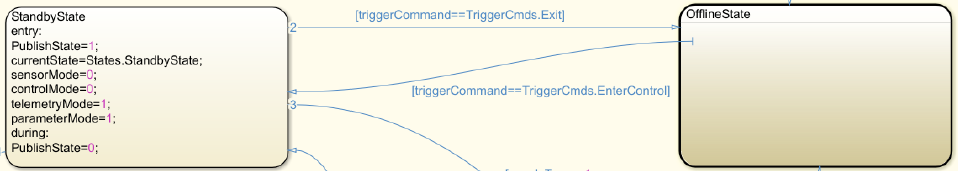
\includegraphics[width=4.68750in]{jira_imgs/1018.png}

\medskip }
\end{minipage} \\ \cdashline{2-2}

 & Actual Result \\
 & \begin{minipage}[t]{15cm}{\footnotesize
\smallskip

\medskip }
\end{minipage} \\ \cdashline{2-2}

 & Status: \textbf{ Not Executed } \\ \hline

6 & Description \\
 & \begin{minipage}[t]{15cm}
{\footnotesize
\smallskip
\textbf{STANDBYSTATE -\textgreater{} DISABLEDSTATE}\\
From the StandbyState, send a start command through the DDS.

\medskip }
\end{minipage}
\\ \cdashline{2-2}


 & Expected Result \\
 & \begin{minipage}[t]{15cm}{\footnotesize
\smallskip
The system transitions into DisabledState after receiving/responding to
DDS command and the wrapper in the PXI real time controller looks for
the configuration file.\\
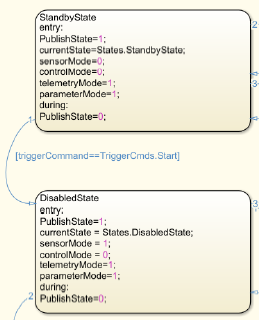
\includegraphics[width=1.79167in]{jira_imgs/1019.png}\\
If the configuration file is invalid or out of range, the system will
transition into a Fault State

\medskip }
\end{minipage} \\ \cdashline{2-2}

 & Actual Result \\
 & \begin{minipage}[t]{15cm}{\footnotesize
\smallskip

\medskip }
\end{minipage} \\ \cdashline{2-2}

 & Status: \textbf{ Not Executed } \\ \hline

7 & Description \\
 & \begin{minipage}[t]{15cm}
{\footnotesize
\smallskip
\textbf{DISABLEDSTATE -\textgreater{} ENABLEDSTATE}\\
From the DisabledState, send an enable state command through the DDS.\\
\textbf{}

\medskip }
\end{minipage}
\\ \cdashline{2-2}


 & Expected Result \\
 & \begin{minipage}[t]{15cm}{\footnotesize
\smallskip
The system transitions into the EnabledState/Stationary substate, the
motor drives are enabled, motor brakes are released and the system is
capable of receiving/responding to DDS commands.\\
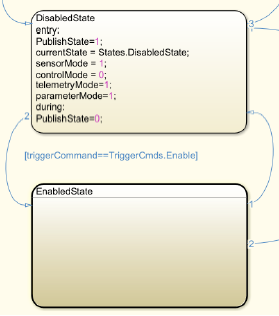
\includegraphics[width=1.79167in]{jira_imgs/1020.png}\\

\medskip }
\end{minipage} \\ \cdashline{2-2}

 & Actual Result \\
 & \begin{minipage}[t]{15cm}{\footnotesize
\smallskip

\medskip }
\end{minipage} \\ \cdashline{2-2}

 & Status: \textbf{ Not Executed } \\ \hline

8 & Description \\
 & \begin{minipage}[t]{15cm}
{\footnotesize
\smallskip
\textbf{FAULTSTATE}\\
If a Fault occurs in any of the other states, the system will
automatically transition to the Fault State. While in the Fault state,
send a clearError command through the DDS.\\
Note: If the fault that occurs goes through the interlock system, reset
the safety relay switch and send a clearError command.

\medskip }
\end{minipage}
\\ \cdashline{2-2}


 & Expected Result \\
 & \begin{minipage}[t]{15cm}{\footnotesize
\smallskip
The system transitions back to the OfflineState/PublishOnly substate and
is not capable of receiving/responding to DDS commands. (Go back to Step
3)\\
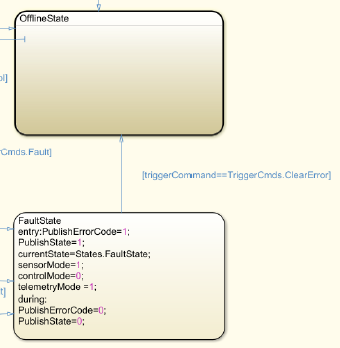
\includegraphics[width=1.79167in]{jira_imgs/1021.png}

\medskip }
\end{minipage} \\ \cdashline{2-2}

 & Actual Result \\
 & \begin{minipage}[t]{15cm}{\footnotesize
\smallskip

\medskip }
\end{minipage} \\ \cdashline{2-2}

 & Status: \textbf{ Not Executed } \\ \hline

9 & Description \\
 & \begin{minipage}[t]{15cm}
{\footnotesize
\smallskip
{Remove the locking pin that so that the CCW moves independently from
the CR.}

\medskip }
\end{minipage}
\\ \cdashline{2-2}


 & Expected Result \\
 & \begin{minipage}[t]{15cm}{\footnotesize
\smallskip

\medskip }
\end{minipage} \\ \cdashline{2-2}

 & Actual Result \\
 & \begin{minipage}[t]{15cm}{\footnotesize
\smallskip

\medskip }
\end{minipage} \\ \cdashline{2-2}

 & Status: \textbf{ Not Executed } \\ \hline

10 & Description \\
 & \begin{minipage}[t]{15cm}
{\footnotesize
\smallskip
The following steps define what the Jupyter Notebook for this test case
implements. Executing the Jupyter notebook is the only actual step that
needs to be executed.

\medskip }
\end{minipage}
\\ \cdashline{2-2}


 & Expected Result \\
 & \begin{minipage}[t]{15cm}{\footnotesize
\smallskip

\medskip }
\end{minipage} \\ \cdashline{2-2}

 & Actual Result \\
 & \begin{minipage}[t]{15cm}{\footnotesize
\smallskip

\medskip }
\end{minipage} \\ \cdashline{2-2}

 & Status: \textbf{ Not Executed } \\ \hline

11 & Description \\
 & \begin{minipage}[t]{15cm}
{\footnotesize
\smallskip
Send a trackStart command to the rotator.~

\medskip }
\end{minipage}
\\ \cdashline{2-2}


 & Expected Result \\
 & \begin{minipage}[t]{15cm}{\footnotesize
\smallskip

\medskip }
\end{minipage} \\ \cdashline{2-2}

 & Actual Result \\
 & \begin{minipage}[t]{15cm}{\footnotesize
\smallskip

\medskip }
\end{minipage} \\ \cdashline{2-2}

 & Status: \textbf{ Not Executed } \\ \hline

12 & Description \\
 & \begin{minipage}[t]{15cm}
{\footnotesize
\smallskip
Send a track command via the pointing component to track in the positive
direction.

\medskip }
\end{minipage}
\\ \cdashline{2-2}


 & Expected Result \\
 & \begin{minipage}[t]{15cm}{\footnotesize
\smallskip

\medskip }
\end{minipage} \\ \cdashline{2-2}

 & Actual Result \\
 & \begin{minipage}[t]{15cm}{\footnotesize
\smallskip

\medskip }
\end{minipage} \\ \cdashline{2-2}

 & Status: \textbf{ Not Executed } \\ \hline

13 & Description \\
 & \begin{minipage}[t]{15cm}
{\footnotesize
\smallskip
{Using the encoders, verify that the CCW and CR are moving
synchronously. (}{If we run the test asynchronously, we just need to
check the CCW and CR are within the 2.2 degrees of each other}{)}

\medskip }
\end{minipage}
\\ \cdashline{2-2}


 & Expected Result \\
 & \begin{minipage}[t]{15cm}{\footnotesize
\smallskip

\medskip }
\end{minipage} \\ \cdashline{2-2}

 & Actual Result \\
 & \begin{minipage}[t]{15cm}{\footnotesize
\smallskip

\medskip }
\end{minipage} \\ \cdashline{2-2}

 & Status: \textbf{ Not Executed } \\ \hline

14 & Description \\
 & \begin{minipage}[t]{15cm}
{\footnotesize
\smallskip
\textbf{{Run High Rotation specific Jupyter Notebook}}

\medskip }
\end{minipage}
\\ \cdashline{2-2}


 & Expected Result \\
 & \begin{minipage}[t]{15cm}{\footnotesize
\smallskip

\medskip }
\end{minipage} \\ \cdashline{2-2}

 & Actual Result \\
 & \begin{minipage}[t]{15cm}{\footnotesize
\smallskip

\medskip }
\end{minipage} \\ \cdashline{2-2}

 & Status: \textbf{ Not Executed } \\ \hline

15 & Description \\
 & \begin{minipage}[t]{15cm}
{\footnotesize
\smallskip
The following steps define what the Jupyter Notebook for this test case
implements. Executing the Jupyter notebook is the only actual step that
needs to be executed.

\medskip }
\end{minipage}
\\ \cdashline{2-2}


 & Expected Result \\
 & \begin{minipage}[t]{15cm}{\footnotesize
\smallskip
The Jupyter notebook controls the system to run through the steps below.

\medskip }
\end{minipage} \\ \cdashline{2-2}

 & Actual Result \\
 & \begin{minipage}[t]{15cm}{\footnotesize
\smallskip

\medskip }
\end{minipage} \\ \cdashline{2-2}

 & Status: \textbf{ Not Executed } \\ \hline

16 & Description \\
 & \begin{minipage}[t]{15cm}
{\footnotesize
\smallskip
With the Camera Rotator and CCW in the Enabled state, send a
\emph{trackStart} command to the rotator.

\medskip }
\end{minipage}
\\ \cdashline{2-2}


 & Expected Result \\
 & \begin{minipage}[t]{15cm}{\footnotesize
\smallskip
The Camera Rotator transitions from the Enabled/Stationary state to the
Enabled/SlewingAndTracking state.

\medskip }
\end{minipage} \\ \cdashline{2-2}

 & Actual Result \\
 & \begin{minipage}[t]{15cm}{\footnotesize
\smallskip

\medskip }
\end{minipage} \\ \cdashline{2-2}

 & Status: \textbf{ Not Executed } \\ \hline

17 & Description \\
 & \begin{minipage}[t]{15cm}
{\footnotesize
\smallskip
Send a \emph{track} command via the pointing component to track in the
positive direction.

\medskip }
\end{minipage}
\\ \cdashline{2-2}


 & Expected Result \\
 & \begin{minipage}[t]{15cm}{\footnotesize
\smallskip
The Camera Rotator starts it's rotation in the positive direction and
the CCW synchronizes with this rotation.

\medskip }
\end{minipage} \\ \cdashline{2-2}

 & Actual Result \\
 & \begin{minipage}[t]{15cm}{\footnotesize
\smallskip

\medskip }
\end{minipage} \\ \cdashline{2-2}

 & Status: \textbf{ Not Executed } \\ \hline

18 & Description \\
 & \begin{minipage}[t]{15cm}
{\footnotesize
\smallskip
Send a \emph{stop} command to the rotator.

\medskip }
\end{minipage}
\\ \cdashline{2-2}


 & Expected Result \\
 & \begin{minipage}[t]{15cm}{\footnotesize
\smallskip
The Camera Rotator and CCW stop their rotation.

\medskip }
\end{minipage} \\ \cdashline{2-2}

 & Actual Result \\
 & \begin{minipage}[t]{15cm}{\footnotesize
\smallskip

\medskip }
\end{minipage} \\ \cdashline{2-2}

 & Status: \textbf{ Not Executed } \\ \hline

19 & Description \\
 & \begin{minipage}[t]{15cm}
{\footnotesize
\smallskip
Send a stopTracking command to the pointing component.

\medskip }
\end{minipage}
\\ \cdashline{2-2}


 & Expected Result \\
 & \begin{minipage}[t]{15cm}{\footnotesize
\smallskip
The pointing component stops sending \emph{track} commands.

\medskip }
\end{minipage} \\ \cdashline{2-2}

 & Actual Result \\
 & \begin{minipage}[t]{15cm}{\footnotesize
\smallskip

\medskip }
\end{minipage} \\ \cdashline{2-2}

 & Status: \textbf{ Not Executed } \\ \hline

20 & Description \\
 & \begin{minipage}[t]{15cm}
{\footnotesize
\smallskip
Send a positionSet command with and angle of 0.0 deg.

\medskip }
\end{minipage}
\\ \cdashline{2-2}


 & Expected Result \\
 & \begin{minipage}[t]{15cm}{\footnotesize
\smallskip
The Camera Rotator and CCW do \textbf{NOT} move.

\medskip }
\end{minipage} \\ \cdashline{2-2}

 & Actual Result \\
 & \begin{minipage}[t]{15cm}{\footnotesize
\smallskip

\medskip }
\end{minipage} \\ \cdashline{2-2}

 & Status: \textbf{ Not Executed } \\ \hline

21 & Description \\
 & \begin{minipage}[t]{15cm}
{\footnotesize
\smallskip
Send a \emph{move} command to rotate to the 0.0 deg position.

\medskip }
\end{minipage}
\\ \cdashline{2-2}


 & Expected Result \\
 & \begin{minipage}[t]{15cm}{\footnotesize
\smallskip
The Camera Rotator and CCW rotate to the 0.0 deg position. The Camera
Rotator publishes the inPosition event.

\medskip }
\end{minipage} \\ \cdashline{2-2}

 & Actual Result \\
 & \begin{minipage}[t]{15cm}{\footnotesize
\smallskip

\medskip }
\end{minipage} \\ \cdashline{2-2}

 & Status: \textbf{ Not Executed } \\ \hline

22 & Description \\
 & \begin{minipage}[t]{15cm}
{\footnotesize
\smallskip
Wait for 120 sec.

\medskip }
\end{minipage}
\\ \cdashline{2-2}


 & Expected Result \\
 & \begin{minipage}[t]{15cm}{\footnotesize
\smallskip
The Camera Rotator and CCW do not move for 120 sec.

\medskip }
\end{minipage} \\ \cdashline{2-2}

 & Actual Result \\
 & \begin{minipage}[t]{15cm}{\footnotesize
\smallskip

\medskip }
\end{minipage} \\ \cdashline{2-2}

 & Status: \textbf{ Not Executed } \\ \hline

23 & Description \\
 & \begin{minipage}[t]{15cm}
{\footnotesize
\smallskip
Send a \emph{trackStart} command to the rotator.

\medskip }
\end{minipage}
\\ \cdashline{2-2}


 & Expected Result \\
 & \begin{minipage}[t]{15cm}{\footnotesize
\smallskip
The Camera Rotator transitions from the Enabled/Stationary state to the
Enabled/SlewingAndTracking state.

\medskip }
\end{minipage} \\ \cdashline{2-2}

 & Actual Result \\
 & \begin{minipage}[t]{15cm}{\footnotesize
\smallskip

\medskip }
\end{minipage} \\ \cdashline{2-2}

 & Status: \textbf{ Not Executed } \\ \hline

24 & Description \\
 & \begin{minipage}[t]{15cm}
{\footnotesize
\smallskip
Send a \emph{track} command via the pointing component in the negative
direction.

\medskip }
\end{minipage}
\\ \cdashline{2-2}


 & Expected Result \\
 & \begin{minipage}[t]{15cm}{\footnotesize
\smallskip
The Camera Rotator starts it's rotation in the negative direction and
the CCW synchronizes with this rotation.

\medskip }
\end{minipage} \\ \cdashline{2-2}

 & Actual Result \\
 & \begin{minipage}[t]{15cm}{\footnotesize
\smallskip

\medskip }
\end{minipage} \\ \cdashline{2-2}

 & Status: \textbf{ Not Executed } \\ \hline

25 & Description \\
 & \begin{minipage}[t]{15cm}
{\footnotesize
\smallskip
Send a \emph{stop} command to the rotator.

\medskip }
\end{minipage}
\\ \cdashline{2-2}


 & Expected Result \\
 & \begin{minipage}[t]{15cm}{\footnotesize
\smallskip
The Camera Rotator and CCW stop their rotation.

\medskip }
\end{minipage} \\ \cdashline{2-2}

 & Actual Result \\
 & \begin{minipage}[t]{15cm}{\footnotesize
\smallskip

\medskip }
\end{minipage} \\ \cdashline{2-2}

 & Status: \textbf{ Not Executed } \\ \hline

26 & Description \\
 & \begin{minipage}[t]{15cm}
{\footnotesize
\smallskip
Send a stopTracking command to the pointing component.

\medskip }
\end{minipage}
\\ \cdashline{2-2}


 & Expected Result \\
 & \begin{minipage}[t]{15cm}{\footnotesize
\smallskip
The pointing component stops sending \emph{track} commands.

\medskip }
\end{minipage} \\ \cdashline{2-2}

 & Actual Result \\
 & \begin{minipage}[t]{15cm}{\footnotesize
\smallskip

\medskip }
\end{minipage} \\ \cdashline{2-2}

 & Status: \textbf{ Not Executed } \\ \hline

27 & Description \\
 & \begin{minipage}[t]{15cm}
{\footnotesize
\smallskip

\medskip }
\end{minipage}
\\ \cdashline{2-2}


 & Expected Result \\
 & \begin{minipage}[t]{15cm}{\footnotesize
\smallskip

\medskip }
\end{minipage} \\ \cdashline{2-2}

 & Actual Result \\
 & \begin{minipage}[t]{15cm}{\footnotesize
\smallskip

\medskip }
\end{minipage} \\ \cdashline{2-2}

 & Status: \textbf{ Not Executed } \\ \hline

\end{longtable}


\newpage
\appendix
%Make sure lsst-texmf/bin/generateAcronyms.py is in your path
\section{Acronyms used in this document}\label{sec:acronyms}
\addtocounter{table}{-1}
\begin{longtable}{p{0.145\textwidth}p{0.8\textwidth}}\hline
\textbf{Acronym} & \textbf{Description}  \\\hline

CR & Change Request \\\hline
CSV & Comma Separated Values \\\hline
GUI & Graphical User Interface \\\hline
IS & Interface Scientist \\\hline
LSST & Large Synoptic Survey Telescope \\\hline
PMCS & Project Management Controls System \\\hline
SLAC & SLAC National Accelerator Laboratory (formerly Stanford Linear Accelerator Center; SLAC is now no longer an acronym) \\\hline
\end{longtable}


\end{document}
